% Created with jtex v.1.0.20
\documentclass{article}
\usepackage{hyperref}
\usepackage{datetime}
\usepackage{graphicx}
\usepackage{natbib}
\bibliographystyle{abbrvnat}

%%%%%%%%%%%%%%%%%%%%%%%%%%%%%%%%%%%%%%%%%%%%%%%%%%
%%%%%%%%%%%%%%%%%%%%  imports  %%%%%%%%%%%%%%%%%%%
\usepackage{amsmath}
\usepackage{amsthm}
\usepackage{framed}
%%%%%%%%%%%%%%%%%%%%%%%%%%%%%%%%%%%%%%%%%%%%%%%%%%
%%%%%%%%%%%%%%%%%%%%%%%%%%%%%%%%%%%%%%%%%%%%%%%%%%
%%%%%%%%%%%%%%%%%%%%  theorem  %%%%%%%%%%%%%%%%%%%
\newtheorem{theorem}{Theorem}[section]
\newtheorem{corollary}{Corollary}[theorem]
\newtheorem{lemma}[theorem]{Lemma}
\newtheorem{proposition}{Proposition}[section]
\newtheorem{definition}{Definition}[section]
\newtheorem{example}{Example}[section]
\newtheorem{remark}{Remark}[section]
\newtheorem{axiom}{Axiom}[section]
\newtheorem{conjecture}{Conjecture}[section]
\newtheorem{observation}{Observation}[section]
%%%%%%%%%%%%%%%%%%%%%%%%%%%%%%%%%%%%%%%%%%%%%%%%%%




% colors for hyperlinks
\hypersetup{colorlinks=true, allcolors=blue}

\newcommand{\logo}{
  \href{https://curvenote.com}{
\includegraphics[width=2cm]{curvenote.png}}
}

\title{Mathematical Physics and Computation}

\author{Haoyu Tang}

\newdate{articleDate}{4}{9}{2026}
\date{\displaydate{articleDate}}

\begin{document}
\maketitle
\begin{center}\logo\end{center}


\section{Linear Operator}

\subsection{Finite-dimensional Vector Space}

\include{mathematical-physics-linear-operators}

\subsubsection{Inner Product Space}

\textit{Note:The development of concepts need to keep extension to infinite analog in mind}

\paragraph{The identity operator and the Kroncker's Delta}

Let $V$ be a vector space endorsed with an inner product $\langle\cdot| \cdot \rangle$ of dimension $n$ and $\beta = \{e_\nu\}$ be an orthonormal basis. Then we can compute the inner product between arbitrary $x,y\in V$ as follows:
\begin{equation}
\langle x | y \rangle  &= \langle e_{\nu} | x \rangle^* \langle e_{\nu} | y\rangle \\ 
&= \langle x | e_{\nu} \rangle \langle e_{\nu} | y\rangle \\
&= \langle x \lvert |e_{\nu} \rangle \langle e_{\nu}|  \rvert y\rangle
\end{equation}
But $\langle x | y \rangle = \langle x | I | y \rangle$, hence we get that

\begin{lemma}[Outer-product decomposition of the identity operator]Let $\{e_{\nu}\}$ be an orthonormal basis for $V$, then:
\begin{equation}
|e_{\nu} \rangle \langle e_{\nu}|=I
\end{equation}

\end{lemma}\begin{framed}
\textbf{\textit{Help!} What is happening here?}\\
\textit{Step 1} We first rewrite inner product as a sum of component-component product. In $\mathbb{C}^3$ for instance,
\begin{equation}
\langle x | y\rangle &= \sum_{\nu} (x^{\nu})^* y^{\nu} \\
&= \sum_{\nu} \langle e_{\nu} | x \rangle^*  \langle e_{\nu} | y \rangle
\end{equation}
Note in the last step we envicted orthonormality of $\{e_\nu\}$. Adopting Einstein notaiton we get the first equality.

\textit{Step 2} We are bascially writing two consecutive inner product $\langle x, \alpha \rangle \langle \beta, y \rangle$ as a bilinear form $\langle x, A y\rangle$ where $A=| \alpha \rangle \langle \beta |$. Consider this example in $\mathbb{R^3}$:

\begin{equation}
\langle x, \alpha \rangle \langle \beta, y \rangle &=
\begin{pmatrix}
x^1 & x^2 & x^3
\end{pmatrix}
\begin{pmatrix}
\alpha^1 \\ \alpha^2 \\ \alpha^3
\end{pmatrix}
\begin{pmatrix}
\beta^1 & \beta^2 & \beta^3
\end{pmatrix}
\begin{pmatrix}
y^1 \\ y^2 \\ y^3
\end{pmatrix} \\
&= 
\begin{pmatrix}
x^1 & x^2 & x^3
\end{pmatrix}
\begin{pmatrix}
\alpha^1 \beta^1 & \cdots & \alpha^1\beta^3 \\
\vdots & & \vdots \\
\alpha^3 \beta^1 & \cdots & \alpha^3\beta^3
\end{pmatrix}
\begin{pmatrix}
y^1 \\ y^2 \\ y^3
\end{pmatrix} \\
\end{equation}

In otherword, we are just invoking associative law(which holds in vector space):
\begin{equation}
(x\alpha^T) (\beta y^T)&=x(\alpha^T \beta) y^T
\end{equation}
where the outer product $\alpha^T \beta=A$.

We denote bilinear forms $x^TAy$ in sandwich notations: $\langle x |A|y\rangle$

\textit{(Step 3)} The only possble opeartor to be sandwitched without changing the result:
\begin{equation}
\langle x|Ay\rangle &= \langle x | y\rangle
\end{equation}
is when $A=I$. We therefore conclude that the outer product $|e_{\nu}\rangle \langle e_{\nu}|$ is the identity. In math notation, this is saying:

\begin{itemize}
\item For orthonormal basis $\{e_{\nu}\}$, we have

\begin{equation}
\sum_{\nu=1}^n e_{\nu}e_{\nu}^T=I
\end{equation}
\end{itemize}
\end{framed}

Now we consider representing $|x\rangle$ in $\beta$:
\begin{equation}
|x\rangle &= (|e_{\nu} \rangle \langle e_{\nu}|) |x\rangle \\
&= |e_{\nu}\rangle \langle e_{\nu}|x\rangle
\end{equation}
Now consider taking the inner product with another basis $e_{\mu}$:
\begin{equation}
\langle e_{\mu}|x\rangle  &=\langle e_{\mu}|e_{\nu}\rangle \langle e_{\nu}|x\rangle
\end{equation}

\subsection{Infinite-dimensional Vector Space}

\subsubsection{Linear Operators}

\paragraph{$L^p$ Space}

\begin{definition}[ space]\textbf{$L^p$}\\
Let $(X,\Sigma, \mu)$ be a measure space and $1\leq p\leq \infty$. The space $L^p(X,\mu)$ is the set of all measurable functions from $X$ to $\mathbb{R}$ or $\mathbb{C}$ such that $\int_X |f(x)|^p d\mu < \infty$.

\begin{itemize}
\item Note $L^p$ is a \textit{normed space} with norm:

\begin{equation}
\|f\|_{L_p}=\left(\int_X |f|^p d\mu\right)^{1/p}
\end{equation}


$p$ can be the symbol $\infty$ with the norm defined as:

\begin{equation}
\|f\|_{L_{\infty}} = \inf\{C\in \mathbb{R}_{\geq 0} : |f(x)|<C, \forall x\}
\end{equation}


\item It is \textit{complete}, hence it is a Banach Space
\end{itemize}

\end{definition}\paragraph{Linear Operators}

\begin{definition}[Linear Operators]Let $T$ be a map betwen two normed space $X$ and $Y$. $T$ is linear if:
\begin{equation}
T(x+\lambda y) = T(x) +\lambda T(y)
\end{equation}
$\forall x,y \in X, \lambda \in K$

\end{definition}If we consider linear functions $f:\mathbb{R}\to \mathbb{R}$, it seems continuity is free since we can always write $T(x)=kx$ hence:
\begin{equation}
\|T(x)-T(x_0)\|=\|k(x-x_0)\|=k\|x-x_0\|
\end{equation}
so we can easily find a delta ball of radius $\frac{\epsilon}{k}$ given an epsilon ball such that the delta ball is mapped into the epsilon ball. More generally we can define bounded operator to make the above logic work:

\begin{definition}[Bounded Operators]Let $T$ be a map betwen two normed space $X$ and $Y$. $T$ is bounded if $\exists C>0$:
\begin{equation}
\|T(x)\|_Y\leq C\|x\|_X
\end{equation}
$\forall x \in X$

\end{definition}\begin{proposition}[Continuous and Bounded are equivalent for Linear Operator]The following are equivalent:

\begin{enumerate}
\item If $X$ and $Y$ are normed spaces and $T:X\to Y$ is a linear map which is continuous from $X$ to $Y$
\item $T$ is bounded
\end{enumerate}

\end{proposition}\begin{proof}\begin{itemize}
\item Suppose $T$ is \textbf{linear and bounded}, $\forall x_0 \in X$, $\forall \epsilon > 0$, consider the open ball around $x_0$ with radius $\epsilon$ $B_{\epsilon}^o$. Then $\forall x\in B_{\epsilon}^o$:
\begin{equation}
\|T(x)-T(x_0)\| &= \|T(x-x_0)\| \\
&\leq C\|x-x_0\|
\end{equation}
Now to make $C\|x -x_0\|<\epsilon$, we need $\|x -x_0\|<\frac{\epsilon}{C}$. Hence $\delta(\epsilon)=\frac{\epsilon}{C}$


\item Suppose $T$ is \textbf{linear and continous}. Then in particular $T$ is continous at $x=0$. We can find a $\delta >0$ such that $\|x\| < \delta \Rightarrow \|T(x)\| < 1$. Now to control arbitrary $x\in X$, we can rewrite $x$ as
\begin{equation}
x=\left(\frac{2}{\delta }\right)\|x\|\left(\frac{\delta x}{2\|x\|}\right)=C\|x\|x'
\end{equation}
Note $\|x'\|=\frac{\delta }{2}\|x\|<\delta$ hence $\|T(x')\|\leq 1$. By linearity $T(x)=T(C\|x\|x')=C\|x\|T(x')$. Thus:
\begin{equation}
\|T(x)\|_Y=C\|x\|\|T(x')\|\leq C\|x\|
\end{equation}
\end{itemize}

\end{proof}It turns out all finite-dimensional linear operator are bounded. However, infinite-dimensional linear operator can easily be unbounded.

\subsubsection{Linear Differential Operator}

\paragraph{The Formal Linear Differential Operator}

We define the differentian opeartor as:

\begin{definition}[Differentiation Opeartor]Let $D:L^2[a,b]\to L^2[a,b]$ be the mapping defined by:
\begin{equation}
D(u)=\frac{d}{dx}u
\end{equation}
for all $u\in L^2[a,b]$

\end{definition}Now we can define the \textit{formal linear operator} by some opeartor algebra:

\begin{definition}[Formal linear differential operator]Let $p(x)$ be any polynomial over $\mathbb{C}$ of positive degree:
\begin{equation}
p(x)=a_\nu x^\nu
\end{equation}
where $a_{\nu}$ are functions of $x$. Define $L:=p(D)$ as the \textbf{formal linear differential operator} that correspond to the \textbf{auxillary polynomial $p$}:
\begin{equation}
L=a_\nu D^{\nu}
\end{equation}
The \textbf{order} of $L$ is given by the order of $p$.

\end{definition}We call it \textit{formal} since we want to contrast with \textit{concrete} linear differential opeartor which is a formal opeartor endorsed with boundary conditions(This convention is used in \textit{Mathematical Physics by Michael Stone and Paul Goldbart}). We can think of the difference between them as:

\begin{itemize}
\item The \textbf{nullspace of formal opeartor} is the space of general solution of homogenous diffferential equation
\item The \textbf{nullspace of concrete operator} is the space of particular solution to homogenous differential equation with boundary conditions
\end{itemize}

We'll explore the nullspace of formal operators with a bit more detail now.

\subparagraph{Nullspace of formal operator}

We first observe something very nice about solutions to homogenous differential equations: they belong to $C^{\infty}$(infinitely differentiable).

\subparagraph{The Bootstrapping Lemma}

\begin{lemma}Let $L$ be a formal operator of order $n$. Suppose the coefficients of the auxillary polynomial are $k$ times continously differentiable($a_{\nu}\in C^k$) then $\forall y\in \mathrm{Null}(L)$, $y$ is at least $k+n$ times contiously differentiable.

\end{lemma}\begin{proof}Suppose $y\in \mathrm{Null}(L)$, note trivially $y\in C^n$. Then:
\begin{equation}
a_0y+a_1y^{(1)}+a_2y^{(2)}...+a_n y^{(n)} &=0 \\
y^{(n)} &= -(b_0y+b_1y^{(1)}+b_2y^{(2)}...\underbrace{b_{n-1}{y}^{n-1}}_{\in C^{\min(k, 1)}})
\end{equation}
Where $b_{\nu}=a_{\nu}/a_{n}$. Now $b_{\nu}\in C^k$ by closedness under polynomial division. Also $y^{(\nu)} \in C^{n -\nu}$ hence the R.H.S is at least one time continously differentiable(the bottle neck being $a_{n -1}y^{(n -1)} \in C^{\min(k, 1)}$). Therefore $y^{(n)}\in C^1$. But this implies $y\in C^{n+1}$ hence we repeat the above argument to get $y^{(\nu)}\in C^{n+1 -\nu}$. The R.H.S has the bottleneck $a_{n -1}y^{(n -1)}\in C^{\min(k, n+1 -(n -1))}=C^{\min(k, 2)}$. We can repeat this procedure $m$ times and yield that $y^{(n)}\in C^{\min(k, m)}$. This means the best we can get is $y^{(n)}\in C^k$ or $y\in C^{n+k}$(after which the coeficient becomes the bottleneck).

\end{proof}\begin{corollary}If the coefficients are in $C^{\infty}$ then $y\in \mathrm{Null}(L)$ are in $C^{\infty}$.

\end{corollary}\subparagraph{Nullspace of $L$ is an $n$-dimensional subspace of $C^{\infty}$}

\paragraph{Linear Independence: Wronskian}

\paragraph{Solving $Ly=0$ with constant coefficients}

\paragraph{$Ly=0$ with general $a_\nu(x)$}

\subsubsection{Inner Product Space}

\paragraph{Distribution and Test Functions}

\subparagraph{Continous Indexing}

\subparagraph{Duality Pairing}

\subparagraph{Exercises}

\paragraph{Formal adjoint}

\paragraph{Concrete Adjoint}

\subparagraph{The Sturm-Liouville Operator}

The \textbf{Sturm-Liouville operator} is a linear differential operator of the form
\begin{equation}
\mathcal L=-\frac{d}{dx}\left(p\frac{d}{dx}y\right)+q\frac{d}{dx}
\end{equation}

We've shown that the Sturm-Liouville opeartor is self-adjoint with appropriate boundary condition in the sense that:
\begin{equation}
\langle u, \mathcal Lv \rangle &= \langle \mathcal L^*u, v \rangle
\end{equation}
hence it is analgous to self-adjoint operator in finite-dimensional vector spaces, which as symmetric matrix representation when the underlying field is real. We now make this connection explicit, i.e., actually constructing the discretized, finite-dimensional matrix representation of the Sturm-Liouville Operator.

\subparagraph{A Discrete Analog}

Let's consider a concrete SL opeartor defined on $[0,1]$ with Dirchlet boundary condition $y(0)=y(1)=0$. Instead of directly discretizing $\mathcal L$, we aim to find a matrix $L$ such that discretizes the quadratic form:
\begin{equation}
F(y)=\int y\mathcal Ly dx \rightarrow \hat y^TL\hat y
\end{equation}
First we note that:
\begin{equation}
\label{func}
F(y) &= \int_0^1 y\left(-\frac{d}{dx}\left(p\frac{d}{dx}y\right) + qy\right) dx \\
&= \int_0^1 -y \frac{d}{dx}\left(p\frac{d}{dx}y\right)dx+\int_0^1 qy^2dx  \\
&= -\left\{\cancel{\left[yp\frac{dy}{dx}\right]_0^1} - \int p\left(\frac{dy}{dx}\right)^2 \right\} + \int_0^1 qy^2dx \\
&= \int_0^1 py'^2 + qy^2
\end{equation}
Now we discretize $y, p, q$ to $N$-dimensional arrays:
\begin{equation}
\hat y &= [y_1,...,y_N] \\
\hat p &= [p_1,...,p_N] \\
\hat q &= [q_1,...,q_N]
\end{equation}
Using forward difference we get:
\begin{equation}
\hat y =\left(\frac{y_{i+1}-y_i}{h}\right)^2
\end{equation}
Rewrite the integral as a finite sum we obtain a discretized version of (\ref{func}):
\begin{equation}
\boxed{\hat F(\hat y)=\sum_{i=1}^N h p_i\left(\frac{y_{i+1}-y_i}{h}\right)^2 +q_iy_i^2}
\end{equation}
Our goal is now to find a matrix $L$ such that $\hat y^TL\hat y=\hat F(\hat y)$. Rewrite $\hat F(\hat y)$:
\begin{equation}
\hat F(\hat y) =\sum_{i=1}^N Np_i(y_{i+1}^2 -2y_{i+1}y_i +y_i^2)+\frac{1}{N}q_iy_i^2
\end{equation}
We can split $L=L_1+L_2$ such that

\begin{enumerate}
\item $\hat y^T L_1 \hat y = \sum_{i=1}^N Np_i(y_{i+1}^2 -2y_{i+1}y_i +y_i^2)$
\item $\hat y^T L_2 \hat y = \sum_{i=1}^N \frac{1}{N}q_iy_i^2$.
\end{enumerate}

\textbf{(Constructing $L_1$)}
Let's first deal with $L_1$. Consider the $2\times 2$block with the upperleft corner at $(i,i)$ that should
represent $Np_i(y_{i+1}^2 -2y_{i+1}y_i +y_i^2)$. This is easy:
\begin{equation}
A_i=Np_i\begin{pmatrix}
1 & -1\\
-1 & 1 \\
\end{pmatrix}
\end{equation}
To assemble $L_1$ we can overlap $A_i$ along the diagonal of $L$ with a stride of 1. Concretely:

\begin{verbatim}
for i=1,...,N -1
    L[i,i] += Np_i
    L[i+1,i+1] += Np_i
    L[i,i+1] -= Np_i 
    L[i+1,i] -= Np_i
\end{verbatim}

\begin{example}A quick example for $N=4$:
\begin{equation}
4\begin{pmatrix}
p_1 & -p_1 & 0 & 0 \\
-p_1 & p_1+p_2 & -p_2 &0 \\
0 & -p_2 & p_2+p_3 & -p_3 \\
0 &  0 & -p_3  & p_3
\end{pmatrix}
\end{equation}

\end{example}\textbf{(Constructing $L_2$)}
$L_2$ is purely diagonal and is easier to derive. Since it only has quadratic term $y_i^2$, at each row $i$ we only need to include $y_i$. Hence:
\begin{equation}
L_2 = \frac{1}{N}\begin{pmatrix}q_1 & & \\
& \ddots & \\
& & q_N
\end{pmatrix}
\end{equation}

\textbf{(Assembly $L_1+L_2$)}
It is clear that $L$ should look like:

\begin{equation}
L=N\begin{pmatrix}
p_1&  -p_1 & & &  \\
-p_1& p_1+p_2 &  -p_2 & &  \\
&  \ddots  &  \ddots &   \ddots &   \\
&  &-p_{N-1} &p_{N-1}+p_{N} & -p_N  \\
& & &-p_N & p_N \\
\end{pmatrix} 
+ 
\frac{1}{N}\begin{pmatrix}q_1 & & \\
& \ddots & \\
& & q_N
\end{pmatrix}
\end{equation}

However, since we are dealing with concrete operators with accompanying domain and boundary condition, we need to encoorperate the Dirchelt boundary condition $y(0)=1, y(1)=0$ into $L$. To do so we need to zero-out the first row and column of $L$. Hence finally we get:

\begin{proposition}The Sturm-Liouville Operator on $[0,1]$ with Dirchlet boundary condition $y(0)=y(1)$ can be discretized as
\begin{equation}
\label{discreteSL}
L=N\begin{pmatrix}
0 &0 & & &  &\\
0 &p_1+p_2 & -p_2& & & \\
&-p_2&  \ddots &\ddots & -p_{N-1}& \\
& & \ddots &-p_{N-1} & p_{N-1}+p_N &0 \\
& & & &0 & 0\\
\end{pmatrix} 
+ 
\frac{1}{N}\begin{pmatrix}0 & & & & \\
& q_2 & & & \\
&  & \ddots& & \\
& & & q_{N-1} & \\
& &  & & 0  \\
\end{pmatrix}
\end{equation}

\end{proposition}We can see that $L$ is indeed a symmetric real matrix(Hermitian)!

\textbf{Numpy Implementation}
This can easily be translated to naive \texttt{numpy} code:

\begin{verbatim}
class SturmLiouville:
    def __init__(self,N, p, q=None, grid='forward'):
        A = np.zeros(shape=(N,N))
        if grid == 'forward':
            for i in range(N -1):
                A[i, i] += p[i]
                A[i+1, i+1] += p[i]
                A[i, i+1] -= p[i]
                A[i+1, i] -= p[i]

        if q is not None:
            I = np.eye(N) 
            L = A + q @ I
        else:
            L = A
        
        # Dirchlet Boundary Condition
            L[0,0]=0.0
            L[0,1]=0.0
            L[1,0]=0.0
            L[N -1,N -1]=0.0
            L[N -1,N -2]=0.0
            L[N -2,N -1]=0.0
        self.L = (L * N ** 2)
        self.N = N

    def solve_eigen(self, top_k=10):
        eval, evec = np.linalg.eig(self.L)
        top_k_idx = np.argsort(eval[eval>0])[:top_k]
        return eval[top_k_idx] , evec[:, top_k_idx], top_k_idx
\end{verbatim}

\textbf{Example: $-\frac{d^2}{dx^2}$ as a Matrix}
We can do a quick example to showcase that $L$ is indeed a discretization of $\mathcal L$.

\begin{example}[-]\textbf{$\frac{d^2}{dx^2}$}\\
We have already seen that the opeartor:
\begin{equation}
T=-\frac{d^2}{dx^2}, D(T)=\{y,Ty \in L^2[0,1]:y(0)=y(1)=0\}
\end{equation}
has eigenvalues and eigenvectors:
\begin{equation}
y_j(x) &=\sqrt{2}\sin j\pi x \\
\lambda_j &= j^2\pi^2
\end{equation}
for $j=1,2,3...$. The problem is that, can we solve a matrix eigenvalue problem to recover exactly the same result?
Indeed we can! Passing $p= -1$ and $q=0$ gets us:
\begin{equation}
L=N\begin{pmatrix}
0 & 0 & &  &  \\
0 & 2 & -1 & &  \\
 & -1 & \ddots & \ddots & \\
& & \ddots & 2 & -1  &\\
& & & -1& 2 & 0\\
& & & & 0 & 0 \\
\end{pmatrix}
\end{equation}

and solving the matrix eigenvalue problem
\begin{equation}
L\hat y &= \lambda \hat y
\end{equation}
 gets us:
\footnote{Since iterative eigensolvers gives eigenvectors of arbitrary magnitude $v_j=a\sin(j\pi(x))$, we need to normalize properly by
1.Ensure $a>0$

\begin{enumerate}
\item Divide by $\sqrt{\sum y_i^2 h}$
\end{enumerate}}

\begin{figure}[!htbp]
\centering
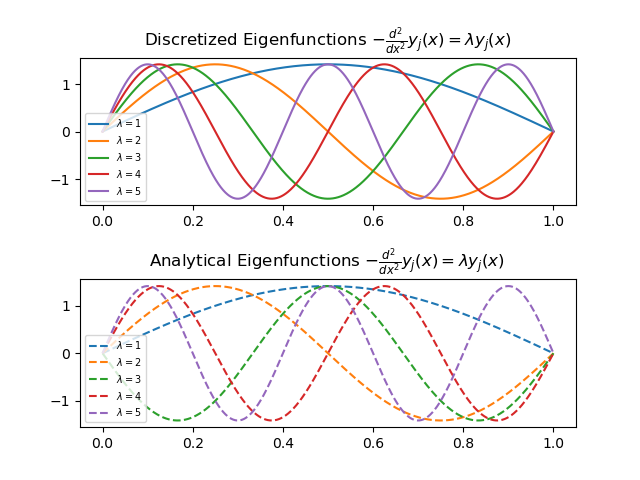
\includegraphics[width=0.7\linewidth]{files/sl_evecs-749bd46b634f4b726002411b1a849030.png}
\end{figure}

\end{example}
%  
% :::{note} Optimizing $x^TAx$ gives $Ax=\lambda x$
% Let $x\in \mathbb{R}^n$, $A\in \mathbb{R^{n\times n}}$ is a **symmetric** matrix, define:
% $$
% F(x)=\frac12 \langle x,Ax \rangle
% $$
% Consider the optimization of $F$ constrained on $\|x\|^2=1$ 
% :::
% 
% We use lagarange multiplier:
% $$
% (Ax)^T+x^TA-2\lambda x^T &=0 \\
% Ax + A^Tx - 2\lambda x &=0 \\
% 2(A-\lambda I)x&=0 \\
% Ax &= \lambda x
% $$ 
% [^diff]
% Subjected to $\|x\|^2=1$. We note that this is an **eigenvalue problem**. 
%

\section{Calculus of Variation}

\subsection{Euler-Lagrange Equation}

\subsubsection{Differential Equation from Physics}

A lot of physical science and engineering is about finding a reduction from a physical problem to differential equations. The newtownian way is to zoom into some local point of the system and derive a set of constraint that holds in the neighborhood. In the case of the vibration of a string, for example, we would find some local segment of string and analyze the tension that acts on it:
\begin{equation}
T(\sin(\theta_1)-\sin(\theta_2)) = m\frac{\partial^2 u}{\partial t^2}
\end{equation}
where $u$ is the vertical displacement from equilibrium. We then take the calculus limit and find out that locally the accelearation of the vertical displacement should be proportional to the curvature. Hence the one-dimensional wave equation:
\begin{equation}
\frac{\partial^2 u}{\partial t^2}=a^2 \frac{\partial^2 u}{\partial x^2}
\end{equation}
\footnote{Here $a$ is a physical parameter intrinsic to the string, i.e., $\sqrt{T}{\rho}$ where $T$ is the tension at equilibrium adn $\rho$ is the density.}

The Lagrangian way is the opposite, we recognize some global objective the system need to be optimized toward, i.e., minimizing the lagragian $L=T -V$ where $T$ is \textit{kinetic energy} and $V$ is \textit{potential energy}. Then, by introduce some perturbation, we extract a constraint which also manifest itself as a differential equation. The following sections descirbes this process in detail.

\begin{framed}
\textbf{Newtonian and Lagrangian Mechanics}\\
\begin{itemize}
\item Newtonian mechanics compute the balance of forces locally and obtain differential equation through

\begin{equation}
F=m\frac{d^2\mathbf{x}}{dt^2}
\end{equation}


\item Lagrangian mechanics translate the physics into some global optimization problem  and reduce to differential equation through the Euler-Lagrange equation

\begin{equation}
\frac{\partial L}{\partial y}- \frac{d}{dx}\frac{\partial L}{\partial y'}=0
\end{equation}
\end{itemize}
\end{framed}

\subsubsection{Functional : A global optimization objective}

A functional in \textit{calculus of variation} is a map from a function to a real number, i.e., $J:C^{\infty} \to \mathbb{R}$. In particular, it mostly comes in some sort of a integral. The simplest form being analgous to that of the lagrangian:

\begin{equation}
\label{basicfunctional}
J[y] = \int_{x_1}^{x_2} f(x,y,y')dx
\end{equation}

The above example suffice to establish the explict connection of (\ref{basicfunctional})to Lagrangian:

\begin{example}[The lagrangian for the vibrating string]Let $u$ be deviation from the equilibrium position

\begin{enumerate}
\item \textbf{The kinetic energy}:

\begin{equation}
T=\frac{1}{2}\int_{0}^L \rho u_t(x,t)^2dx
\end{equation}


where $L$ is the length of the string


\item \textbf{The potential energy}:

\begin{equation}
V=\frac{1}{2}k\int_{0}^L {1+u_x^2} dx
\end{equation}

\footnote{It is tempting for some of us who are not trained as a physics student to write the potential energy as $\frac12 \left(\int_a^b \sqrt{1+u_x^2}dx\right)^2$. The rationale is as follows: if we pause at a moment and straigten the vibrating string as a line. Then we observe how much elongation had happened and use hooke's law on the entire string. This is physically wrong since the elongation happens inhomogenously hence we have to apply hooke's law locally and integrate. Also mathematically,
\begin{equation}
\left(\int f\right)^2 =\int f^2
\end{equation}
iff $f$ is some constant function. The general relatinoship can be obtained from Cauchy-Shwarz inequality by taking $f=\sqrt{1+u_x^2}$ and $g=1$
\begin{equation}
\left(\int_0^L \sqrt{1+u_x^2}\right)^2 \leq \int_0^L 1+u_x^2 dx
\end{equation}}
\end{enumerate}

The lagrangian is hence:
\begin{equation}
L=\int_0^L \frac{1}{2} \left(\rho u_t(x,t)^2 - k(1+u_x^2)\right)
\end{equation}

\begin{figure}[!htbp]
\centering
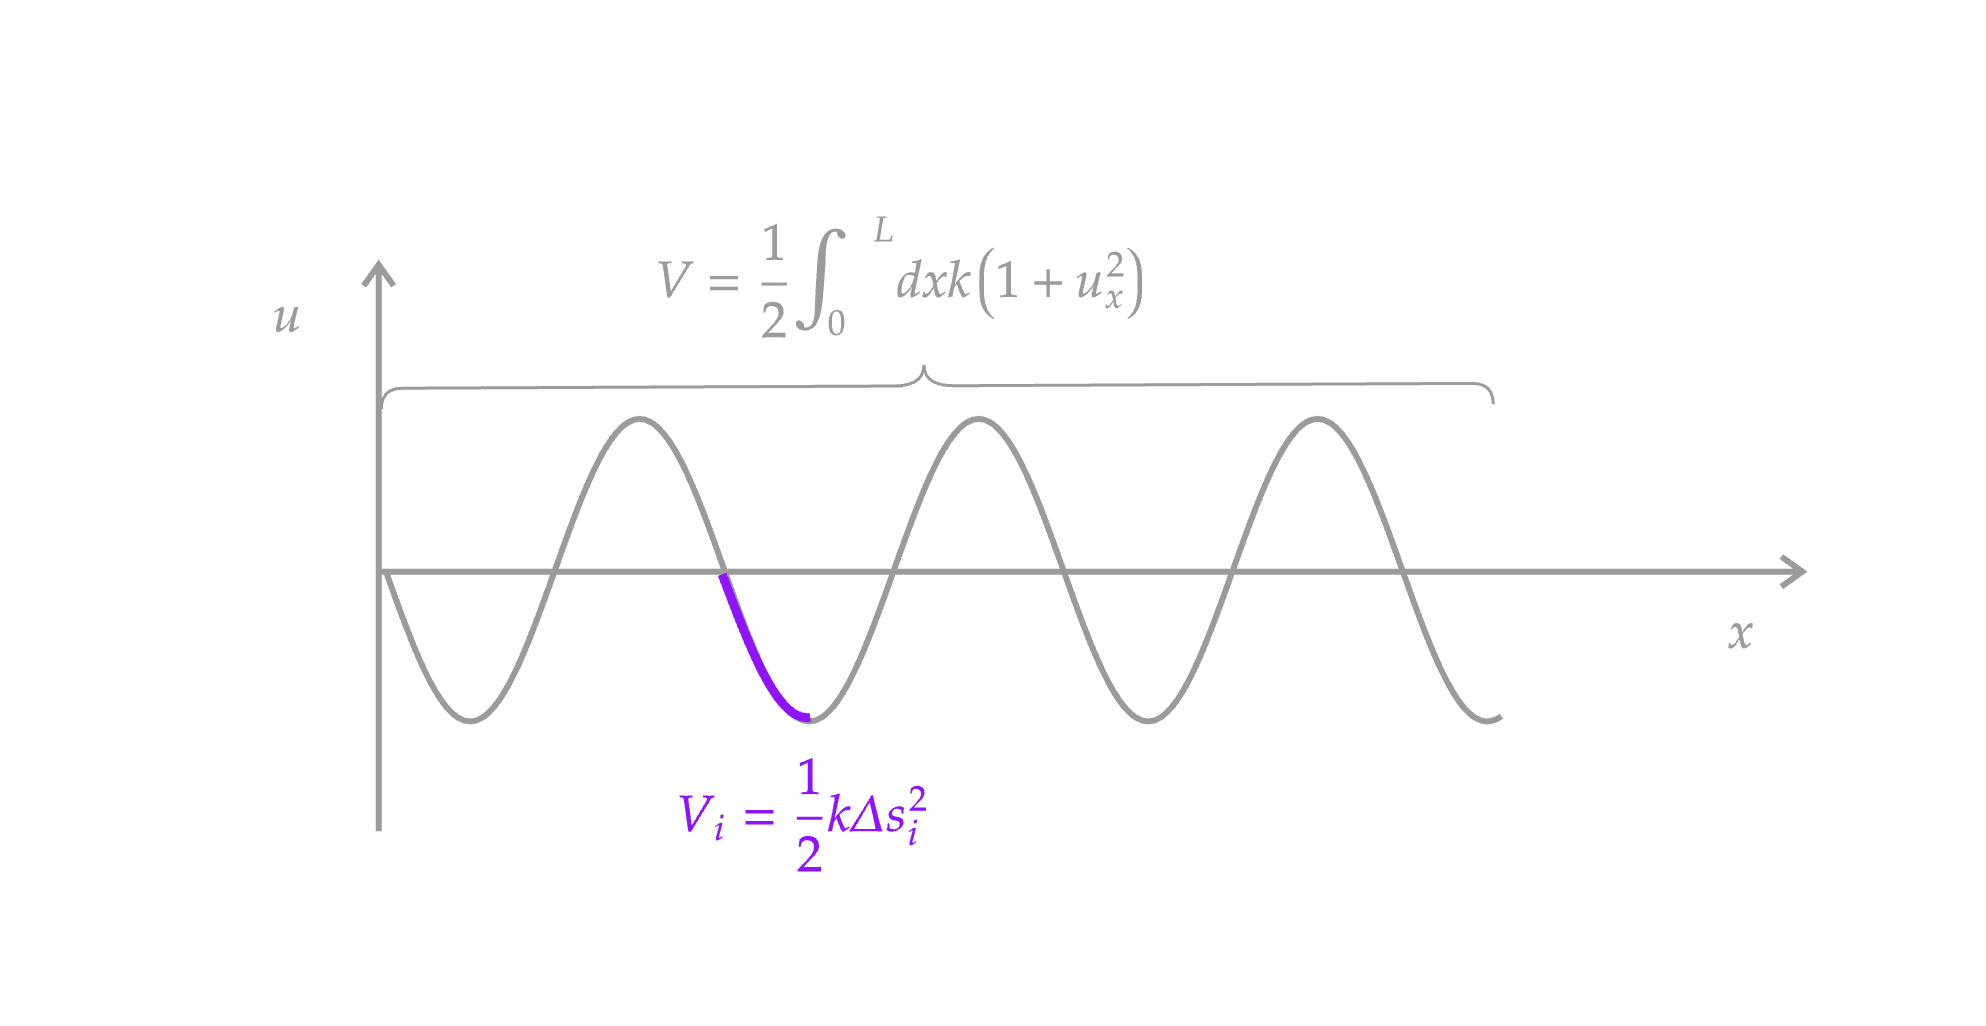
\includegraphics[width=0.7\linewidth]{files/vs-89ee0e6d488b170eecb5d0f3a41cc551.png}
\caption*{The potential energy of a vibrating string.}
\end{figure}

\end{example}We now scrutinize how exactly we optimize (\ref{basicfunctional}).

\subsubsection{Euler-Lagrange Equation}

\begin{theorem}[Euler-Lagrange Equation]$y$ is a stationary point for
\begin{equation}
J[y] = \int_{x_1}^{x_2} f(x,y,y^{(1)},...,y^{(n)})dx
\end{equation}
iff:
\begin{equation}
\boxed{\frac{\partial f}{\partial y} -\frac{d}{dx}\left(\frac{\partial f}{\partial y'}\right)=0}
\end{equation}
The boxed equation is known as the \textbf{Euler-Lagrange Equation}

\end{theorem}\subsubsection{Discretized Euler-Lagrange Equation}

\subsubsection{First Integral}

\begin{definition}[First Integral]Suppose
\begin{equation}
y^{(n)}=f(x,y,y^{(1)},...,y^{(n-1)})
\end{equation}

is an ordinary differential equation of order $n$. We can define an equivalent $n$-dimensional system by letting:
\begin{equation}
y_1 &= y \\
y_2 &= y^{(1)} \\
\vdots \\
y_{n} &= y^{(n-1)}
\end{equation}
Denote by:
\begin{equation}
\frac{dy_i}{dx}=f_i(x,y_1,...,y_n)
\end{equation}
Now suppose $f$ is:

\begin{enumerate}
\item Continous about $x,y_1,...,y_n$
\item Continuously differentialbe about $y_1,...,y_n$
\end{enumerate}

Define  the \textit{first integral} of the $n^{\text{th}}$-order problem to be a function $I=I(x,y_1,...,y_n)$ that also satisfies the above two requirements , and furthermore has the definitive property:
\begin{equation}
I(x,y_1,...,y_n)=\text{Constant}
\end{equation}
along solution curves $\Gamma=(y_1(x),y_2(x),...,y_n(x))$ with the constant determined by the solution curve.

\end{definition}We are confronted by the higher-order ordinary differential equation:
\begin{equation}
\label{ele}
\frac{\partial f}{\partial y} -\frac{d}{dx}\left( \frac{\partial f}{\partial y'}\right)=0
\end{equation}
The compute the first integral of this equation is to rewrite the above to obtain an equation of the form:
\begin{equation}
\frac{d}{dt}I(x,y,y',...)=0
\end{equation}
The strategy is to compute the difference between (\ref{ele}) and the exact differential:
\begin{equation}
\frac{df}{dx}=\frac{\partial f}{\partial x} + \sum_{j\geq 0}\frac{\partial f}{\partial y^{(j)}}\frac{dy^{(j)}}{dx}=\frac{\partial f}{\partial x} +\frac{\partial f}{\partial y}\frac{dy}{dx}+\frac{\partial f}{\partial y^{(1)}}\frac{dy^{(1)}}{dx}+\cdots
\end{equation}
If we multiply (\ref{ele}) by $y'$ and subtract the two equations we get:

\begin{equation}
\frac{df}{dx}-y'\left\{\frac{\partial f}{\partial y} - \frac{d}{dx}\left( \frac{\partial f}{\partial y'}\right)\right\} =\frac{\partial f}{\partial x} + \textcolor{cyan}{y''\frac{\partial f}{\partial y'}+ y'\frac{d}{dx}\left( \frac{\partial f}{\partial y'}\right)}-\sum_{j\geq 2}\frac{\partial f}{\partial y^{(j)}}\frac{dy^{(j)}}{dx}
\end{equation}

\begin{framed}
\textbf{The particular form that allows easy first integral}\\
If we assume $f$ is only dependent on $y,y'$, the above becomes $f(y,y')$, then
\begin{equation}
\sum_{j\geq 2}\frac{\partial f}{\partial y^{(j)}}\frac{dy^{(j)}}{dx} &= 0\\ 
\frac{\partial f}{\partial x} &=0
\end{equation}
\end{framed}

Now:
\begin{equation}
\frac{df}{dx}-\underbrace{y'\left\{\frac{\partial f}{\partial y} - \frac{d}{dx}\left( \frac{\partial f}{\partial y'}\right)\right\}}_{0}&= \frac{d}{dx}\left(y'\frac{\partial f}{\partial y'}\right)
\end{equation}
Hence:
\begin{equation}
\frac{d}{dx}\left(f-y'\frac{\partial f}{\partial y'}\right)=0
\end{equation}
We have sucesfully obtained the first inetgral:
\begin{equation}
I(y,y)=f-y'\frac{\partial f}{\partial y'}
\end{equation}

\subsubsection{Exercises}

\paragraph{Euler-Lagrange Equation for Multiple Independent Variables}

\textbf{Prove} that:

\begin{theorem}[Euler-Lagrange Equation]Consider the functional
\begin{equation}
J[y]=\int f(x_1,x_2,...,x_n,y_{x_1},y_{x_2},...,y_{x_n})d\mathbf{x}
\end{equation}
Show that the stationary is acheived iff:
\begin{equation}
\frac{\partial f}{\partial y} - \sum_{i}\frac{d}{dx}\left(\frac{\partial f}{\partial y_{x_i}}\right)
\end{equation}

\end{theorem}
\bigskip
\centerline{\rule{13cm}{0.4pt}}
\bigskip

\paragraph{Fermat's Principle \footnote{From Dr. P.Draper's homework problems for PHYS 508(\textit{Mathematical Physics I}) at UIUC.}}

\begin{framed}
\textbf{Fermat's Principle}\\
The path taken by a ray of light between any two point makes stationary the travel time between those points.
\end{framed}

We also define:

\begin{definition}[Refractive Index]A medium is characterized by the speed of light traveling through. Specifically, the refractive index is defined by $n=\frac{c}{\text{speed of light traveling in the medium}}$

\end{definition}\begin{framed}
\textbf{\textbf{Problem 1} Light Propagtes in Straight Line in Homogenous Media}\\
\begin{enumerate}
\item \textbf{Show that light propagates along a stragiht line in homogenous media.}
\end{enumerate}
\end{framed}

\begin{framed}
\textbf{\textit{Solution}}\\
Since $n$ is independent of position in homogenous media, make stationary the travel time is equivalent to make stationary the length of the path taken. Now the problem is equivalent to optimizing:
\begin{equation}
\int_{x_1}^{x_2} \sqrt{1+y'^2}dx
\end{equation}
Note:
\begin{equation}
f_y = 0 \quad f_y' = \frac{y'}{\sqrt{1+y'^2}}
\end{equation}
The Euler-Lagrange equation is, therefore:
\begin{equation}
\frac{}{}
    \frac{d}{dx}\left[ \frac{y'}{\sqrt{1+y'^2}}\right] &= 0 \\
    \frac{y'}{\sqrt{1+y'^2}} &= C_1
\end{equation}
Note the L.H.S is a non-constant function of $y'$, hence:
\begin{equation}
y'= C_2 \Longrightarrow y=C_2x+C_3
\end{equation}
\end{framed}

\begin{framed}
\textbf{\textbf{Problem 2} Snell's Law}\\
Consider the propagation of light from a flat slab of glass of refractive index $n_1$ into to
another with refractive index $n_2$. By examining paths that need not be differentiable
at the flat interface, establish Snell's law:
\begin{equation}
n_1\sin(\theta_1) = n_2\sin(\theta_2)
\end{equation}
\end{framed}

\begin{framed}
\textbf{\textit{Solution}}\\
We consider the first point at $(x_1, 0)$, the second point at $(x_2,y_2)$ where $x_1<0<x_2$. The time taken is hence:
\begin{equation}
\int_{x_1}^{x_2} \frac{1}{v(x)}\sqrt{1+y'^2}dx
\end{equation}
where:
\begin{equation}
v(x)=
\begin{cases}
    c/n_1 &\text{if } x<0 \\
    c/n_2 &\text{if } x>0
\end{cases}
\end{equation}
The Euler-Lagrange equation is:
\begin{equation}
0 + \frac{d}{dx}\left( \frac{y'}{v(x)\sqrt{1+y'^2}} \right)=0
\end{equation}
Hence:
\begin{equation}
\frac{y'}{v(x)\sqrt{1+y'^2}} =C
\end{equation}
For $x<0$, we have:
\begin{equation}
\frac{1}{v(x)}\frac{y'}{\sqrt{1+y'^2}} = \frac{n_1}{c}\sin(\theta_1) = C_1
\end{equation}
For $x>0$, we have:
\begin{equation}
\frac{1}{v(x)}\frac{y'}{\sqrt{1+y'^2}} = \frac{n_2}{c}\sin(\theta_2) = C_2
\end{equation}
Hence:
\begin{equation}
n_1\sin(\theta_1)=n_2\sin(\theta_2)
\end{equation}
\textbf{Question:} If we flip the axis we would get $n_1\cos\theta_1=n_2\cos\theta_2$, why is that wrong?
\end{framed}

\begin{framed}
\textbf{\textbf{Problem 3} General Snell's law}\\
A planar light ray propagates in an layered medium with refractive index $n(x)$. Use Fermat's principle to establish a generalized Snell's law:
\begin{equation}
n(x)\sin(\psi(x))=\text{constant}
\end{equation}
by finding the equation for stationary paths for
\begin{equation}
F_1=\int n(x)\sqrt{1+y'^2}dx
\end{equation}
(Here the prime denotes differentiation with respect to x.) Repeat this exercise with $x,y$ swapped by finding a similar equation for the stationary paths of
\begin{equation}
F_2=\int n(y)\sqrt{1+y'^2}dx
\end{equation}
By using suitable definitions of the angle of incidence $\psi$, in each case show that the two formulations of the problem of a layered medium give physically equivalent answers.
(In the second formulation you will find it easiest to use the first integral.)
\end{framed}

\paragraph{Drums and Membranes \footnote{From Dr. P.Draper's homework problems for PHYS 508(\textit{Mathematical Physics I}) at UIUC.}}

The shape of a distorted drumskin is described by the
function $h(x, y)$, which gives the height to which the point $(x, y)$ of the flat undistorted drumskin is displaced.

\begin{framed}
\textbf{\textbf{Problem 1} Area of distorted drumskin}\\
Show that the area of the distorted drumskin is equal to
\begin{equation}
A[h] = \int dxdy \sqrt{1 + \partial_x h^2 + \partial_y h^2}
\end{equation}
\end{framed}

\begin{framed}
\textbf{\textit{Solution}}\\
Consider the area differntial $dA=ds_x ds_y$ where $ds_x=\sqrt{1+\partial_x h^2}dx$ and $ds_y=\sqrt{1+\partial_y h^2}dy$ hence
\begin{equation}
dA=\sqrt{1+\partial_x h^2 + \partial_y h^2 + (\partial_x h\partial_y h)^2}dxdy
\end{equation}
since $\partial_x h\partial_y h\in \mathcal{O}(d\rho^2)$ where $d\rho = \sqrt{dx^2 + dy^2}$ we can drop it. As desired.
\end{framed}

\begin{framed}
\textbf{Area for small distortion}\\
Show that for small distortions, the area reduces to
\begin{equation}
\label{afsd}
   A[h]=\frac{1}{2}\int dxdy |\nabla h|^2 + \text{constant}
\end{equation}
\end{framed}

\begin{framed}
\textbf{\textit{Solution}}\\
Recall the generalized binomial theorem:
\begin{equation}
(1+x)^{\alpha}=1+\alpha x + \frac{\alpha(\alpha-1)}{2!}x^2+\cdots + \frac{\alpha(\alpha-1)...(\alpha-n+1)}{n!}x^n + \cdots
\end{equation}
for $|x|<1$.
As a result:
\begin{equation}
(1+x)^{1/2}=1+\frac12 x + \mathcal{O}(x^2)
\end{equation}
Assume a small perturbation, in particular, assume $|\nabla h|^2 \ll 1$, then
\begin{equation}
\sqrt{1+|\nabla h|^2} = 1 + \frac12 |\nabla h|^2 +  \mathcal{O}(|\nabla h|^4)
\end{equation}
As a result,
\begin{equation}
A[h]=\frac12 \int dxdy |\nabla h|^2 + \underbrace{\int dxdy}_{\text{constant}}
\end{equation}
\end{framed}

\begin{framed}
\textbf{\textbf{Problem 3}}\\
Show that if $h$ satisfies the two-dimensional Laplace equation then $A$ is stationary with
respect to variations that vanish at the boundary.
\end{framed}

\begin{framed}
\textbf{\textit{Solution}}\\
We need that the Euler-Lagrange equation for (\ref{afsd}) is equivlanet to the tow-dimensional Laplace equation. That is simple: let $f(x,y,h, h_x,h_y)=h_x^2 + h_y^2$,
\begin{equation}
\frac{\partial f}{\partial h} + \frac{d}{dx}\left(\frac{\partial f}{\partial h_x}\right) + \frac{d}{dy}\left(\frac{\partial f}{\partial h_y}\right) &= 0 \\
 0 + 2\left(\frac{dh_x}{dx} +  \frac{dh_x}{dx}\right) &= 0\\
 \nabla^2 h &=0
\end{equation}
\end{framed}

\begin{framed}
\textbf{\textbf{Problem 4}}\\
Suppose the drumskin has mass $\rho_0$ per unit area, and surface tension $T$. Write down
the Lagrangian controlling the motion of the drumskin and derive the equation of
motion that follows from it.
\end{framed}

\begin{framed}
\textbf{\textit{Solution}}\\
The kinetic term is given by:
\begin{equation}
T=\frac12 \int_{\Omega} dxdy \rho_0h_t^2
\end{equation}

The potential term is: \footnote{The key to solve this problem is actually to realize that surface tension has the dimension $[F]/[L]=[E]/[L]^2$, in otherword, surface tension is precisely the perunit potential energy due to ``stretching''/``distorsion'' by construction.}
\begin{equation}
V=\int_{\Omega} dxdy T|\nabla h|^2
\end{equation}

Hence the lagrangian is:
\begin{equation}
L &= T-V \\
&= \int_{\Omega} dxdy \left\{\frac12 \rho_0h_t^2 - T|\nabla h|^2 \right\}
\end{equation}

Computing the various derivatives:
\begin{equation}
\frac{\partial L}{\partial h}=0 \quad \frac{\partial L}{\partial h_t}=\rho_0 h_t \quad \frac{\partial L}{\partial h_x}=-2Th_{x} \quad \frac{\partial L}{\partial h_y}=-2Th_{y}
\end{equation}
\end{framed}

\subsection{Generalizations}

This section focuses on more general cases. In particular,

\begin{enumerate}
\item \textbf{Multiple Constraint}, i.e., in the case of

\begin{equation}
J=\int f(x,y_1,y_2,...,y_n,\dot y_1, \dot y_2,...,\dot y_n, \ddot y_1,...)
\end{equation}


\item \textbf{Variable Endpoints}
In previous cases, we used the key assumption that:
\end{enumerate}

\begin{framed}
\textbf{Fixed Endpoint Assumption}\\
The perturbation $\delta y$ is 0 at endpoints, hence all boundary/surface terms arising from integartion by parts may be ignored.
\end{framed}

We now relax this assumption but rather work out boundary conditions based on the stationary condition with variable endpoints. This assumption can in turn be applied to the resulting differential equations.

\begin{enumerate}[resume]
\item \textbf{Constrained Optimization} Often, the minimization of the action is subjected to physcial constraint. For instance, in the famous \textit{catenary problem}, we need to fix the length of the hanging chain.
\end{enumerate}

\subsubsection{Multiple Constraint}

\subsubsection{Variable Endpoints}

\subsubsection{Constraint Optimization}

\subsubsection{Exercises}

\paragraph{Elastic Rods}

\begin{framed}
\textbf{Elastic Rods}\\
\begin{itemize}
\item The \textbf{elastic energy per unit length} of a bent steel rod is given by

\begin{equation}
\frac{1}{2}\frac{YI}{R^2}
\end{equation}


Here Y is the \textit{Young's modulus} of the steel and $I$ is the moment of inertia of the rod's cross section about an axis through its centroid and perpendicular to the plane in which the rod is bent.
\end{itemize}

\begin{figure}[!htbp]
\centering
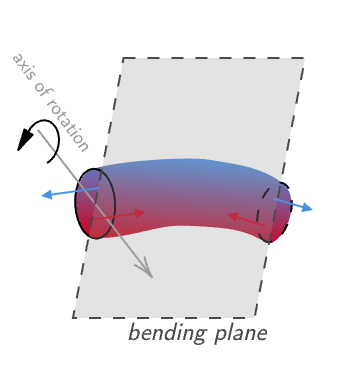
\includegraphics[width=0.375\linewidth]{files/bending_beam-3f593e81e849dc20a7466f2be18f704f.png}
\caption*{Bending beam and the axis of rotation associated with the moment of  inertia $I$}
\end{figure}

\begin{itemize}
\item Let us assume the rod is only slightly bent into the yz plane and lies close to the z axis. R is the radius of curvature due to the bending, related to the curvature by

\begin{equation}
\frac{1}{R}=\kappa = |T_z|
\end{equation}


where $T$ is the unit tangent vector to the rod.
\end{itemize}

\subparagraph{Problem 0}

Show that the elastic energy can be approximated by:
\begin{equation}
\boxed{U[y]=\int_0^L \frac12 \left\{ \frac{1}{2} YI(y'')^2 \right\}dz}
\end{equation}

\subparagraph{Problem 1}

The rod is used as a column which supports a compressive load $Mg$ directed along the z axis (which is vertical). Show that :

\textbf{(a)} when the rod buckles slightly (i.e. bends with both ends remaining on the z axis) the
total energy, including the gravitational potential energy of the loading mass M, can be
approximated by
\begin{equation}
\boxed{U[y]=\int_0^L \left\{ \frac{YL}{2} (y'')^2 - \frac{Mg}{2}(y')^2\right\}dz}
\end{equation}

\textbf{(b)} By considering deformations of the form
\begin{equation}
y(z)=\sum_{n=1}^{\infty} a_n\sin(\frac{n\pi z}{L})
\end{equation}
show that the column is unstable to buckling and collapse once
\begin{equation}
Mg \geq \frac{\pi^2}{L^2}YI
\end{equation}

\subparagraph{}
\end{framed}

\begin{framed}
\textbf{Solution to Problem 0}\\
We need a little lemma(or recall from Calculus I):
\begin{equation}
\kappa = \frac{y''}{(1+y'^2)^{3/2}}
\end{equation}

For small perturbation $|y'|\ll 1$ hence $(1+y'^2)^{\frac32} \approx 1$ hence
$\kappa = \frac{1}{R}=(y'')$. Squaring it we have :
\begin{equation}
\frac{1}{R^2}=(y'')^2
\end{equation}
Hence:
\begin{equation}
dU=\frac12 YI (y'')^2 dz
\end{equation}
Integrating get us the desired result.

\begin{proof}[Proof of lemma]If we imagine we traverse along a curve $\Gamma$, the accelearation would be:
\begin{equation}
r''(z) &= \frac{d}{dz}\left(\frac{dr}{dz}\right) \\
&=  \frac{d}{dz}\left(\frac{ds}{dz}T\right)  \\
&= \frac{d^2s}{dz^2}T + \frac{ds}{dz}\frac{dT}{dz}
\end{equation}
Note that
\begin{equation}
\left\langle T, \frac{dT}{dz}\right\rangle=0
\end{equation}
since $|T|=1$. Therefore $r''(z)$ can be decomposed to a tangential component $\frac{d^2s}{dz^2}T$ and a centrepetal component $\frac{ds}{dz}\frac{dT}{dz}$.
Also, $\frac{dT}{dz}$ is co-linear with our quanitty of interest
\begin{equation}
\frac{dT}{dz}=\frac{dT}{ds}\frac{ds}{dz}
\end{equation}
Therefore:
\begin{equation}
\boxed{r''(z)= \frac{d^2s}{dz^2}T + \left(\frac{ds}{dz}\right)^2 \frac{dT}{ds}}
\end{equation}
We can isolate the centrepetal component by apply a cross product:
\begin{equation}
T\times r''(z) &= T \times \left(\frac{ds}{dz}\right)^2\frac{dT}{dz}
\end{equation}
Now :

\begin{enumerate}
\item (LHS) $T=(1,0,y')/ds$, hence $r''(z) = (0,0,y'')$. Hence the cross product is:

\begin{equation}
\frac{1}{\sqrt{1+y'^2}} (1,0,y')^T \times (0,0,y'')  = \frac{1}{\sqrt{1+y'^2}}(0,y'',0)^T
\end{equation}


\item (RHS) Since $T, \frac{dT}{dz}$ are orthogonal to each other and both lie in the x-z plane, we have:

\begin{equation}
T \times \left(\frac{ds}{dz}\right)^2\frac{dT}{dz} =  \left(\frac{ds}{dz}\right)^2 \textcolor{brown}{\left|\frac{dT}{dz}\right|} (0,1,0)^T
\end{equation}
\end{enumerate}

Now combining the above two equations, we get:
\begin{equation}
\frac{y''}{\sqrt{1+y'^2}}=\left(\frac{ds}{dz}\right)^2  \left|\frac{dT}{dz}\right|
\end{equation}
As desired.

\end{proof}
\end{framed}

\begin{framed}
\textbf{Solution to Problem 1}\\
\begin{figure}[!htbp]
\centering
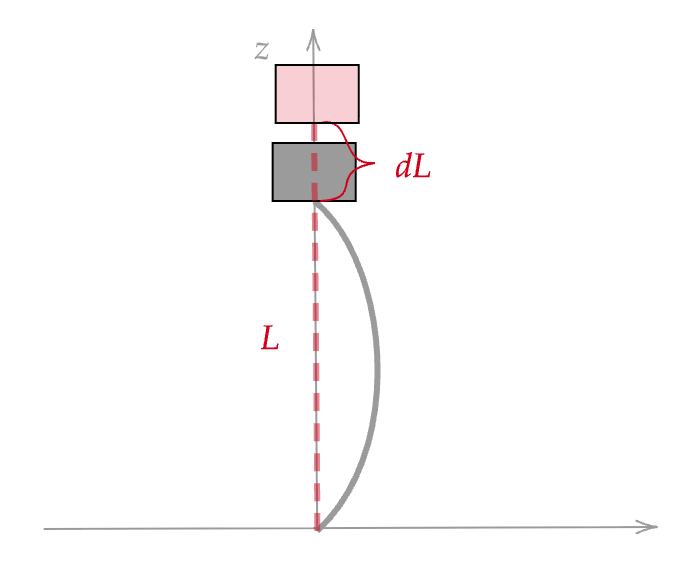
\includegraphics[width=0.7\linewidth]{files/euler_problem-85a6acb1fc4f4cee1ea1426b81e9491a.png}
\end{figure}

(a) Consider the schemetic above. Suppose $y=0$ for $z\in (L -dL,L)$, then
\begin{equation}
L+dL&=\int_0^L \sqrt{1+y'^2}dz \\ 
&\approx \int_0^L 1 + \frac{1}{2}y'^2dz\\
&= L + \int_0^L \frac{1}{2}y'^2dz
\end{equation}
Hence $dL=\int_0^L \frac{1}{2}y'^2$. If we consider the gravitational potential energy to be 0 at $h=L$, then the gravitational potential energy becomes:
\begin{equation}
-\int_0^L \frac{1}{2}y'^2dz
\end{equation}
the negative sign is there to account for compression. Combining with the result from problem 0 we get as desired.

(b) The Euler-Lagrange equation for the total energy functional is:
\begin{equation}
-\frac{d}{dx}\frac{\partial f}{\partial y'}+\frac{d^2}{dx^2}\frac{\partial f}{\partial y''} &= 0 \\
Mgy^{(2)}+YIy^{(4)} &= 0
\end{equation}

Consider a series solution of the form:
\begin{equation}
y(z)=\sum_{n=1}^{\infty} a_n\sin(\omega_n z)
\end{equation}
where $\omega_n = \frac{n\pi}{L}$. We have:

\begin{equation}
\widehat{\frac{\delta J}{\delta f}} &= \sum_{n=1}^{\infty}  b_n \sin(\omega_n z) \\
&= \sum_{n=1}^{\infty}\underbrace{a_n(YI\omega_n^4-Mg\omega_n^2)}_{b_n}\sin(\omega_n z)
\end{equation}

Hence a trivial solution is $a_n=0, \forall n\geq 1$ which corresponds to a \textit{stable, stiff rod}.

The rod buckles if, the trivial solution is no longer a local minimum, i.e., the hessian is no longer positive-definite. We need to find the hessian in this case.

Define the hessian in the spectral space as:

\begin{equation}
\widehat H = 
\begin{pmatrix}
\frac{\partial b_{1}}{\partial a_1} & \frac{\partial b_{1}}{\partial a_2} & \cdots \\
\frac{\partial b_{2}}{\partial a_1} & \frac{\partial b_{2}}{\partial a_2} & \cdots \\
\vdots  & & \ddots \\
\end{pmatrix}
\end{equation}

which in our case is already diagonalized:

\begin{equation}
\widehat H = \mathrm{diag}(\{(YI\omega_n^4-Mg\omega_n^2)\}_{n=1}^{\infty})
\end{equation}

Local minimum requires positive-definiteness, which is :
\begin{equation}
YI\omega_n^4 - Mg\omega_n^2 &> 0  \\
M &< \frac{YI}{g}\omega_n^2
\end{equation}

Picking $n=1$(smallest eigenvalue) satisfies the last inequality.
\begin{equation}
\boxed{M < \frac{YI\pi^2}{g L^2}}
\end{equation}

As desired.
\end{framed}

\section{Function Space}

\subsection{Ｃ\textsubscript{2}𝛑 Space}

\subsubsection{Fourier Basis $e^{ikt}$}

**$C_{2\pi}$  is a space of  continuous functions that is $2\pi$-periodic **. This is precisely the space of functions we are going to expand by fourier series. This chapter is dedicated to show that:

\begin{theorem}[  Space is Spanned by Fourier Basis]\textbf{$C_{2\pi}$}\\
$C_{2\pi}$ is an infinite-dimensional vector space spanned by $\{e^{ikt}\}_{k\in\mathbb{Z}}$. It is also an inner product space endorsed with the inner product:
\begin{equation}
\langle f,g \rangle = \frac{1}{2\pi}\int_{0}^{2\pi} fg^*dt
\end{equation}

\end{theorem}where $g^*$ denotes the \textit{complex conjugate} of $g$.

An elementary observation is that  $\{e^{ikt}\}_{k\in\mathbb{Z}}$ is orthonormal:

\begin{equation}
\frac{1}{2\pi}\int_0^{2\pi}e^{ik_1t}e^{-ik_2t}=\delta_{k_1k_2}
\end{equation}

\begin{proof}Since
\begin{equation}
\frac{1}{2\pi}\int_0^{2\pi}e^{ik_1t}e^{-ik_2t} &= \frac{1}{2\pi}\int_0^{2\pi}e^{i(k_1-k_2)t}
\end{equation}
\begin{equation}
\frac{1}{2\pi}\int_0^{2\pi}e^{i(k_1-k_2)t} = \frac{1}{2\pi}\int_0^{2\pi}\cos(k_1-k_2)t + i\sin(k_1-k_2)t
\end{equation}
If $k_1=k_2$ then it's clear we get 1. Otherwise, since both cosine and sine component above have period $\frac{2\pi}{k_1 -k_2}$ hence $2\pi$ is always a multiple:
\begin{equation}
\frac{1}{2\pi}\int_0^{2\pi}e^{i(k_1-k_2)t}=(k_1-k_2)\underbrace{\int_0^{2\pi}\cos(t)}_{0}+i(k_1-k_2)\underbrace{\int_0^{2\pi} \sin(t)}_{0}
\end{equation}

\end{proof}For arbitary $f:\mathbb{R}\to \mathbb{C}$, if we compute the representation using the infinite basis like what one would do in finite vector space, one would get:
\begin{equation}
\label{fe}
f=\sum_{k\in\mathbb{Z}}\langle f, \exp(ikt)\rangle \exp(ikt)
\end{equation}
This is known as the \textit{Fourier Series}.

\begin{framed}
\textbf{Infinite-dimensional Vector Space}\\
Note although (\ref{fe}) looks like the orthonormal basis expansion in finite-dimensional vector space, such expansion is not guaranteed to be valid by linear algebra theorems. In particular, we need to ensure (\ref{fe}) converges and it converges to $f$.
\end{framed}

So, in otherword, in order to shown we can do fourier expansion(that is, regarding $C_{2\pi}$ as an inner product space endorsed with the $L_2$ inner product), we would have to show its convergence for arbitrary $f\in C_{2\pi}$ first.

\subsubsection{Convergence of Fourier Series}

\paragraph{Theoretical Framework: The Overall Idea}

The overall theoretical framework is

\begin{framed}
\textbf{Big Idea}\\
First consider the infinity norm
\begin{equation}
\|f\|_{\infty}=\sup_t |f|
\end{equation}
Equip $C_{2\pi}$ with the iniftity norm to obtain the Banach Space $(C_{2\pi}, \|\cdot\|_{\infty})$  \footnote{A Banach space is a normed complete vector space}. Then show a weaker form of convergence -- \textbf{Convergence in Abel's Sense} in the Banach space. Finally, since different norms essentially agree with each other, we note that Hilbert Space$(C_{2\pi}, \langle\cdot, \cdot, \rangle_{2})$ inherits the same sense of convergence. This justifies fourier expansion:
\begin{equation}
f=\sum_{k\in\mathbb{Z}}\langle f, \exp(ikt)\rangle \exp(ikt)
\end{equation}

\begin{figure}[!htbp]
\centering
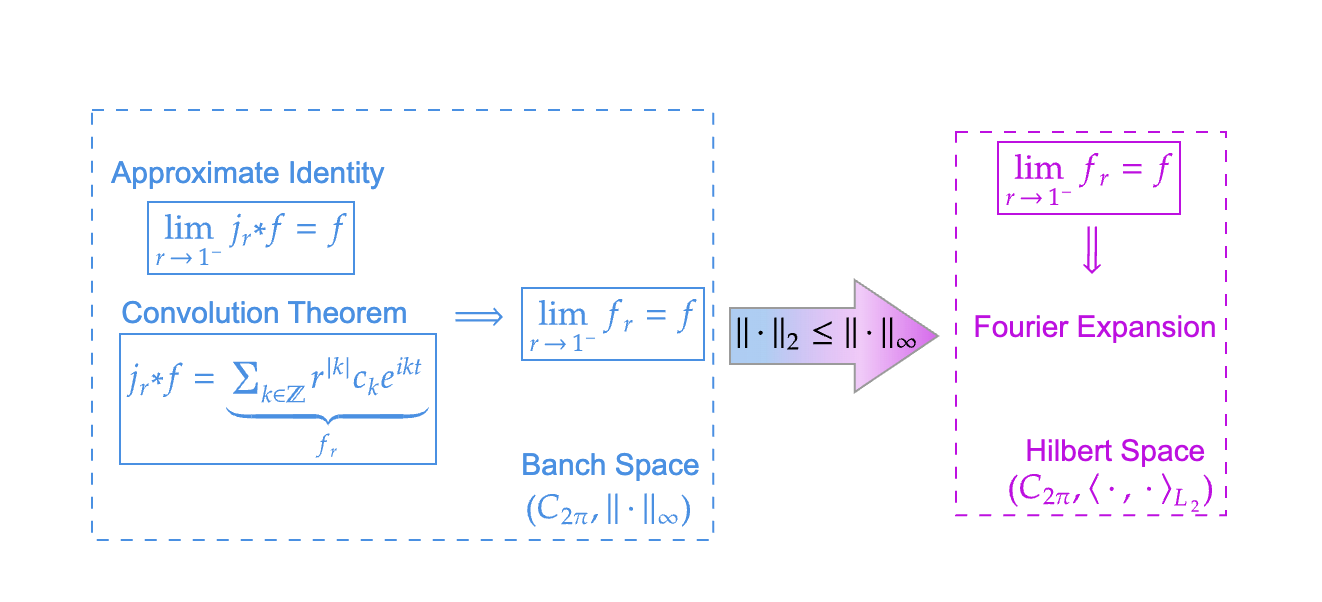
\includegraphics[width=0.7\linewidth]{files/convergence_of_fouri-3fbfbe8d21f6e4000ab45bb3f05154bc.png}
\end{figure}
\end{framed}

\paragraph{Convergence in Abel's Sense}

\begin{figure}[!htbp]
\centering
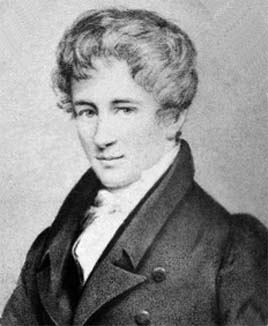
\includegraphics[width=0.7\linewidth]{files/Niels_Henrik_Abel-c40d66306f3721b227d2dd8e2dcabb34.jpg}
\caption*{The famous Norwegian Mathematician Niels Henrik Abel. Quite a good-looking fella ei? Probably everyone's first encoutner would be \textbf{Abel's test} from Calculus, i.e. if $\sum_k a_k$ is convergent, then $\sum_k a_kb_k$ is convergent iff $b_k$ is \textit{monotone} and \textit{bounded}.}
\end{figure}

\begin{definition}[Abel Summation]Consider a constant-valued series $\sum_k a_k$, the corresponding Abel's summation transform it into a power series $\sum_k a_k r^k$. We say $\sum_k a_k$ converges to to $c$ \textit{in the Abel's sense} if
\begin{equation}
\lim_{r \to 1^-}\sum_{k=1}^{\infty} a_k r^k = c
\end{equation}
where $r\to 1^ -$ denotes left limit.

\end{definition}\textit{Rmk. Normal convergence implies Abel's convergence}

\begin{proof}[Normal convergence implies Abel’s convergence ⏩]\textbf{Want}: $\forall \epsilon >0$, $\exists \delta >0$
s.t. $\forall r > 1 -\delta$ we have $\left|\lim_{k\to \infty}\sum_{j=1}^k a_jr^j - c\right|<\epsilon$.

Denote the partial sum as:
\begin{equation}
s_k :=\sum_{j=1}^k a_j
\end{equation}

The goal is to use $\delta$ to control the following quanitity
\begin{equation}
E:=\left|\lim_{k\to \infty}s_j - c\right|
\end{equation}

To do so, we would like to utillize the fact the series is convergent. One way to do so is  manipulate the quantity such that $s_j -c$ appears somewhere:
\begin{equation}
\left|\lim_{k\to \infty}s_j - c\right| &= \left|\lim_{k\to \infty}\sum_{j=1}^k (\textcolor{orchid}{s_j}-\textcolor{pink}{s_{j-1}})r^j - c\right| \\
&= 
\left|\textcolor{orchid}{\lim_{k\to \infty}\sum_{j=1}^k s_jr^j} -  \textcolor{pink}{\lim_{k\to \infty}\sum_{j=1}^{k-1} s_jr^{j+1}} - c\right| \\
&= 
\left| \lim_{k\to\infty}\left[\textcolor{orchid}{s_kr^k} + (\textcolor{orchid}{1}-\textcolor{pink}{r})\sum_{j=1}^{k-1}s_jr^j\right]-c\right|
\end{equation}
Note that

\begin{enumerate}
\item $\lim_{k\to \infty}s_kr^k = 0$ since we know $\lim_{k\to \infty}s_k$ exists and for $|r|<1$, we have $\lim_{k\to\infty}{r^k}=0$ hence by standard limit product law we have

\begin{equation}
\lim_{k\to \infty}s_kr^k=\lim_{k\to \infty}s_k\lim_{k\to \infty}r^k=0
\end{equation}


\item We can write $c$ akin to the form of the term $(\textcolor{orchid}{1} -\textcolor{pink}{r})\sum_{j=1}^{k -1}s_jr^j$, i.e.

\begin{equation}
c=(1-r)\frac{c}{1-r}=(1-r)\lim_{k\to\infty}\sum_{j=1}^k cr^j
\end{equation}
\end{enumerate}

Hence the quantity we want to control becomes:
\begin{equation}
E=\left| (1-r)\sum_{j=1}^{\infty} (s_j-c)r^j\right|
\end{equation}
Intuitively, for small $j$, $s_j -c$ can be large but then we can make the quantity small by picking sufficiently small $\delta=1 -r$. On the otherhand, as the series converge, the tail terms $(s_j -c)$ can be arbitraily small by definition. To convey such idea mathematically, we use a common technique which is to split the series and control the leading and the tail sum respectively:
\begin{equation}
E &= \left| (1-r)\sum_{j=1}^{N} (s_j-c)r^j + (1-r)\sum_{j=N+1}^{\infty} (s_j-c)r^j\right| \\
&\leq \left| (1-r)\sum_{j=1}^{N} (s_j-c)r^j \right| +  \left|(1-r)\sum_{j=N+1}^{\infty} (s_j-c)r^j\right| \\
&\leq  (1-r)\sum_{j=1}^{N} |s_j-c|r^j  +  (1-r)\sum_{j=N+1}^{\infty} |s_j-c|r^j
\end{equation}

\begin{enumerate}
\item For the tail sum, we notice that, by the convergence of the sequence $s_j$, we can pick an $N$ such that $\forall j > N$, $|s_j -c|<\epsilon/2$. Hence:

\begin{equation}
(1-r)\sum_{j=N+1}^{\infty} |s_j-c|r^j &\leq \frac{\epsilon}{2}(1-r)\sum_{j=N+1}^{\infty} r^j \\ 
&= \frac{\epsilon}{2}
\end{equation}


\item For the leading sum, we would like to control:

\begin{equation}
(1-r)\sum_{j=1}^{N} |s_j-c|r^j&\leq \epsilon/2 \\
\end{equation}


if we let $M:=(1 -r)\sum_{j=1}^{N} |s_j -c|$, then $\sum_{j=1}^{N} |s_j -c|r^j \leq M$, then:

\begin{equation}
(1-r)\sum_{j=1}^{N} |s_j-c|r^j\leq (1-r)M = \delta M
\end{equation}


Hence we obtained the requirement on $\delta$:

\begin{equation}
\delta \leq \frac{\epsilon}{2M}
\end{equation}


As desired.
\end{enumerate}

\end{proof}\paragraph{Algebra}

Recall that we can construct vector space(denoted $V$) from fields(denoted by $\mathbb{F}$) by stacking elements from the field together. Valid operators include addition of vector and scalar multiplications. \textit{Algebra} takes one more step and introduce ``vector-vector'' multiplications:

\begin{definition}[Algebra]An \textbf{algebra} is a vector space equipped with a binary operatation $V\times V\to V$ that is \textit{commutative}, \textit{associative} and \textit{distributive}.

\end{definition}In this section, we show that the infinite dimensional vector space $C_{2\pi}$ spanned by $\{e^{ik\pi}\}_{k\in\mathbb{Z}}$ equipped with convolution

\section{Measure Theory}

\subsection{Measure}

It will be inevitable to step on some measure \& integration theory in dealing with \textit{Partial Differential Equations} and \textit{Stochastic Processes}. This chapter acts as a brief introduction.

\paragraph{$\sigma$-Algebra}

\subparagraph{Motivation}

In physics, the task of finiding ``volume'' is ubquitous. For instance in computing mass, charge, the integral would resemble:
\begin{equation}
\int (\cdot ) dV
\end{equation}
In some sense, this $dV$ is a function $dV:E\to \mathbb{R}$ which computes the volume of $E\subset \mathbb{R}^n$, a tiny control volume we are interested in.  It would be very natural to ask for this function to satisfy:

\begin{definition}[Measure]Suppose $X$ is a set. Let $\mu: A \to \mathbb{R}$ where $A\in P(X)$ such that:

\begin{itemize}
\item \begin{equation}
\mu(\varnothing)=0
\end{equation}


\item \textbf{(countable additivity)} $E_1,E_2,....$ is a countable inifnite sequence of disjoint, then:

\begin{equation}
\mu(\cup_j E_j)=\sum_j \mu(E_j)
\end{equation}


Then we call $\mu$ a measure.
\end{itemize}

\end{definition}The question would be, when can we find such a function. Trivially we can obtain such property by sending every $A$ to 0. However, for more practical purposes of modeling the world, we would like nicer properties. In particular, let's consider this compeletly reasonable demand on $\mathbb{R}^n$.

\subsubsection{Construction of Measure}

\paragraph{The big picture}

The general idea of constructing measure is, in crude terms:

\begin{enumerate}
\item Find a collection of set that has a clear notion of size
\item Make the collection closed in finite set operations by generating an algebra on the collection.
\item Approximate arbitrary subsets using element in the algebra, hence get a notion of size on arbtirary subsets
\item Make the notion of size truely a measure by restricting to a special collection of subset.
\end{enumerate}

More concretely the collection of set with clear notion of size need to have a certain structure called \textit{elementary collection of set}(denoted by $\mathcal E$).  \textit{Elementary collection} has a special property: it can be promoted to an algebra $\mathcal A$ by disjoint union. Now the notion of size on $\mathcal E$ can be exteneded to the algebra $\mathcal A$, creating a so-called \textit{pre-measure} which possess \textit{countable additivity} on $\mathcal A$. Then the process of approximating arbitrary set using elementary class
is called the construction of an \textit{outer-measure}. During the process, we looses \textit{countable additivity} as it is reduced to \textit{countable subadditivity}. Finally we obtain a true \textit{measure} by restricting the \textit{outer-measure} on a special collection of subset called the \textit{Caratheory $\sigma$-algebra}.

Observe how the notion of size ripens:
\begin{equation}
\text{Stage 1: $\boxed{|\cdot|:\mathcal E \to \mathbb{R}^+}$} 
&\longrightarrow \text{Stage 2: $\boxed{\mu_0: \mathcal A \to  \mathbb{R}^+}$} \\ 
&\longrightarrow \text{Stage 3: $\boxed{\mu^* : P(X)\to \mathbb{R}^+}$} \\ 
&\longrightarrow \text{Stage 4: $\boxed{\mu: S \to \mathbb{R}^{+}}$}
\end{equation}

\begin{enumerate}
\item \textit{Stage 1 to 2}: Expand the domain to ensures closedness and obtains \textit{countable-additivity}; Lacks the ability to take arbtirary subset as input
\item \textit{Stage 2 to 3}: Expand the domain to arbitray subset but as a cost \textit{countable additivity} deterioates to \textit{countable subadditivity}.
\item \textit{Stage 3 to 4}: Shrink the domain; This is now a \textbf{complete measure}
\end{enumerate}

\paragraph{Elementary collection and pre-measure}

\begin{definition}[Elementary Collection of set]An \textbf{elementary collection} of set is a collection of set $\mathcal E \in P(X)$ such that:

\begin{enumerate}
\item \textbf{(Contains null)} $\varnothing \in \mathcal E$
\item \textbf{(Closed under intersection)} If $E,F\in \mathcal E$ then $E\cap F\in \mathcal E$
\item \textbf{(Closed by disjoint union under complement)} If $F\in \mathcal E$ then exists disjoint subsets $E_j\in \mathcal E$ such that $F^c = \cup_j E$
\end{enumerate}

\end{definition}\paragraph{Outer Measure}

So how do we actually construct measures no matter what set we are working on?(Though in this book we are really interested in just $\mathbb{R}^n$). A general guidline is:

\begin{enumerate}
\item Find some \textit{elementary set} $\mathcal{E}$ where premeasure is defined on the disjoint uniont of $\mathcal{E}$.
\item Define the measure of arbitrary subset $A\in P(X)$ as the the size of ``smallest'' cover of $A$ using the elementary set:
\end{enumerate}
\begin{equation}
\label{omfml}
\inf \left\{\sum_{\nu=1}^{\infty} \rho(E_{\nu}): E_{\nu}\in \mathcal{E}, A\subset \bigcup_{\nu=1}^{\infty} E_{\nu}\right\}
\end{equation}
More generally we can define an \textit{outer measure} as follows:

\begin{definition}[Outer Measure]\label{omdf}An outer measure on an non-empty set $X$ is a function $\mu^* : P(X)\to [0,\infty]$ such that:

\begin{itemize}
\item $\mu^*(\varnothing)=0$
\item If $A\subset B$, then $\mu^*(A)<\mu^*(B)$
\item $\mu^*(\cup_{\nu}A_{\nu})\leq \sum_{\nu} \mu^* (A_{\nu })$
\end{itemize}

\end{definition}We note that property (2),(3) are both derived properties of measure. So we can think the definition of outer measure as a relaxation of measure: take out countable additvity and adds back two derived property. In addition,  We note that (\ref{omfml}) obeys Definition~\ref{omdf}

\begin{framed}
\textbf{Exercise}\\
Show that (\ref{omfml}) indeed defines an outer measure Definition~\ref{omdf}.
\end{framed}

How do we then obtain measure from outer measure? We note that what outer measure lacks is finite additivity, so we can further ask, is there a collection of subset $\mathcal {M}\subset P(X)$ such that $\mu^*$ is actually finitey additive? The answer is actually YES! However this seems rather arbitrary:
\begin{equation}
\mathcal M = \{A\subset X: \mu^*(F)=\mu^*(F-A)+\mu^*(A\cap F), \forall F \subset X\}
\end{equation}
We call elements of $\mathcal M$ \textbf{$\mu^*$-measureable}. In plain English, this saying $A$ can ``split measure'' arbitrary $F\subset X$ by measuring the intersection and the complement separetly and add them together.

\begin{theorem}[Carathéodory’s Theorem]If $\mu^*$ is an outer measure of $X$ then

\begin{enumerate}
\item the collection of \textbf{$\mu^*$-measureable} sets:

\begin{equation}
\mathcal M = \{A\subset X: \mu^*(F)=\mu^*(A^c \cap F)+\mu^*(A\cap F), \forall F \subset X\}
\end{equation}


is a $\sigma$-algebra.


\item $\mu^*|_{\mathcal M}$ is a \textbf{complete measure}
\end{enumerate}

\end{theorem}We first show a small lemma:

\begin{lemma}[ is closed under finite union and ]\textbf{$\mathcal M$$\mu^{*}$ is finitely additive on $\mathcal M$}\\
Let $\mu^{*}$ be an outer measure:

\begin{enumerate}
\item Suppose $A,B\in \mathcal M$ then

\begin{equation}
A\cup B\in \mathcal M
\end{equation}


\item Suppose $A,B\in \mathcal M$, $A\cap B=\varnothing$

\begin{equation}
\mu^{*}(A \cup B) = \mu^*(A)+\mu^*(B)
\end{equation}
\end{enumerate}

\end{lemma}\begin{proof}[proof of lemma]1.(\textbf{$\mathcal M$ is closed under finite union}) It suffice to show that $A \cup B$ split measure every subset in $X$. That is, $\forall F\subset X$
\begin{equation}
\mu^*(F)=\mu^*(F\cap(A\cup B)) + \mu^*(F\cap(A\cup B)^c)
\end{equation}
Since $\mu^*$ has subadditivity by definition, we only need to show:
\begin{equation}
\mu^*(F)\geq \underbrace{\textcolor{red}{\mu^*(F\cap(A\cup B))} + \textcolor{blue}{\mu^*(F\cap(A\cup B)^c)}}_{I}
\end{equation}
where we denoted the quantity to be bounded as $I$. Now note that we can expand the two term again by subadditivity to get:
\begin{equation}
\textcolor{red}{\mu^*(F\cap A \cap B) + \mu^*(F\cap A \cap B^c)+\mu^*(F\cap A^c \cap B)} + \textcolor{blue}{\mu^*(F\cap A^c \cap B^c)}\geq I
\end{equation}
Now we note that $B\in \mathcal M$ hence $B$ can split measure any set, including $F\cap A\subset X$ and $F\cap A^c \subset X$. Hence:
\begin{equation}
\mu^*(F\cap A) +\mu^*(F \cap A^c)\geq I
\end{equation}
But $A \in \mathcal M$ therefore:
\begin{equation}
\mu^*(F)\geq I
\end{equation}

2.(\textbf{$\mu^{*}$ is finitely additive on $\mathcal M$})
First use that $A\in \mathcal M$
\begin{equation}
\mu^*(A\cup B) &= \mu^*((A\cup B)\cap A) +  \mu^*((A\cup B)\cap A^c) \\
&= \mu^*(A\cup (A\cap B))  +  \mu^*(A^c \cap B)
\end{equation}
Now use disjointness to conclude: $A\cap B=\varnothing, A^c \cap B = B$ hence:
\begin{equation}
\mu^*(A\cup (A\cap B))  +  \mu^*(A^c \cap B) &= \mu^*(A)+\mu^*(B)
\end{equation}

\end{proof}\begin{proof}[proof of Carathéodory]We only need to upgrade ``finite'' to ``countable'' in the previous argument.

\end{proof}\subsubsection{Casestudy: Lebesgue-Stieltjes Measure}

The most useful set that we would like to equip a measure with is, unarguably, the real numbers $\mathbb{R}$.

\paragraph{Starting Point: The half-intervals}

Recall that we would start with an elementary collection that has a clear notion of size. We define the \textbf{h-intervals}:
\begin{equation}
H=\{(a,b]:a<b, a,b\in \mathbb{R}\}
\end{equation}

We define a terminology here:

\begin{definition}[Borel Sets]Let $X$ any metric space, the $\sigma$-algebra genereated by the family of open sets in $X$ is called the \textbf{Borel $\sigma$-algebra}, denoted by $\mathcal B_{X}$

\end{definition}Another terminology:

\begin{definition}[Elementary Decomposition]Suppose $A\in \mathcal A$, since $\mathcal A=\mathcal M(H)$ we can find finite disjoint h-intervals $\{I_j\}_{j=1}^N=\{(a_j,b_j]_j\}_{j=1}^N$ such that:
\begin{equation}
A=\bigcup_{j=1}^N I_j
\end{equation}
Then $\{I_j\}$ is an \textbf{elementary decomposition} of $A$.

\end{definition}We define size on $H$ as follows:

\begin{framed}
\textbf{Notion of Size on h-intervals}\\
Let $F:\mathbb{R}\to\mathbb{R}$ be increasing and right-continous, let $(a,b]\in H$, then:
\begin{equation}
|(a,b]|=F(b)-F(a)
\end{equation}
Note when $F(x)=x$, we get the common notion of length of interval.
\end{framed}

The next step is to extend this notion of size to $\mathcal A=\mathcal M(H)$.

\paragraph{Step 1: Construction of a premeasure}

Now we have an algebra $\mathcal A$ where elements of the algebra $A\in \mathcal A$ has an elementary decomposition $A=\{I_j\}$ to h-intervals $I=(a_j,b_j]$, which is equipped with a notion of size $b_j -a_j$. A natural way to define the notion of size for $A$ is hence:
\begin{equation}
\mu_0(A) = \sum_{j=1}^N |I_j| =\sum_{j=1}^N F(b_j)-F(a_j)
\end{equation}
We claim that $\mu_0$ is actually a \textit{pre-measure} on $\mathcal A$.

\begin{proposition}Let $F:\mathbb{R}\to\mathbb{R}$ to be a right-continuous, increasing function. Define $\mu_0$ as
\begin{equation}
\mu_0 : \mathcal A &\to \mathbb{R} \\
\bigcup_{j=1}^N A &\mapsto \sum_{j=1}^N [F(b_j)-F(a_j)]
\end{equation}
where $\{I_j\}=\{(a_j,b_j]\}$ is an elementary decomposition. Then $\mu_0$ is a premeasure on $\mathcal A$.

\end{proposition}\begin{proof}[ is a pre-measure]\textbf{$\mu_0$}\\
We first need to show that $\mu_0$ is actually well-defined\footnote{Note that in definiting a notion of size $\mu_0$ on $A\in \mathcal A$, we requires $A$ to have a concrete representation $\cup_j I_j$. If the result is independent on
how we choose this representation(i.e. different elementary decomposition$\{I_j\}$), then this notion of size is indeed fundamentally correct. Otherwise if $\mu_0$ is dependent on how we choose representation, then it is not a credibe notion of size. Such ``representational invariance'' is called \textit{well-definedness} in mathematics.}. Then we illustrate:

\begin{enumerate}
\item Empty set has zero measure
\item Non-negativity
\item Finite additivity
\item Countable additivity
where only $(1),(2),(4)$ is truely required. But $(3)$ is used in the proof of $(4)$.
\end{enumerate}

\end{proof}

\include{mathematical-physics-measurable-functions}

\section{Partial Differential Euqations}

\subsection{Introduction}

\include{mathematical-physics-introduction}

\subsection{Elementary Methods}

\include{mathematical-physics-conservation-laws}

\include{mathematical-physics-wave-equation}

\subsubsection{Poisson Equation}

\begin{framed}
\textbf{Interactive Visualization !}\\
This notebook contain interactive visualization that needs binder connection. Please click the \textbf{power button on the top right corner} before you start reading ! Establishing the connection and building the container takes a while, so clicking it before you read would make sure the interactive code to be ready to run when you scroll on to them.
\end{framed}

\paragraph{2D Poisson Equation}

Let $\Omega \subset \mathbb{R}^2$, we consider the Poisson equation with homogenous boundary condition:

\begin{definition}[2D Poisson Equation with Homogenous Boundary Condition]\begin{equation}
\label{2dpoihb}
  -\Delta u &= f(x,y) \qquad (x,y)\in \Omega \\
  u(x,y) &= 0 \qquad (x,y)\in \Gamma_1 \\
  \frac{\partial u}{\partial \nu}(x,y) &= 0 \qquad (x,y)\in \Gamma_1
\end{equation}

\end{definition}where $\Gamma_1\cup \Gamma_2 = \partial \Omega$ such that both $\Gamma_1, \Gamma_2$ is measure-zero. $\nu$ is the outward normal vector.

\paragraph{Spectral Method}

Let
\begin{equation}
u(x,y)=\sum_{-\infty<p,q<\infty} a_{pq}  \exp(i(px +qy))
\end{equation}
Which has:
\begin{equation}
\Delta u = \sum_{-\infty<p,q<\infty} a_{pq}
\end{equation}
Also let the fourier transform of $f(x,y)$ be $\mathcal F (f(x,y))=F(p,q)$.

\paragraph{Finite-Element Method(FEM)}

\subparagraph{The Tent Function}

We consider the

\subparagraph{Viualizing the Tent Basis}

\begin{framed}
\textbf{Tip}\\
If you have not do so, click the power button on the top right corner.
After everything builds up, you can click the start button ▶️. You should see two sliders showing up below.

\begin{itemize}
\item The resolution slider determines how ``dense'' these tent basis are in filling the domain. Lower resolution means larger and less tents and vice versa.
\item The position slider let you adjust which particular basis function you are watching. In otherword, where the ``tent'' is located in the domain $\Omega$
\end{itemize}
\end{framed}

%  We define:
% :::{prf:definition} Dirchlet Integral
% Let $u\in C^2(\Omega), v\in C^{\infty}(\Omega)$, define the bilinear form on $H^1(\Omega)$ to be
% $$
% a(u,v) := \int_{\Omega}\nabla u \nabla v
% $$
% :::

We can show that:

\begin{proposition}Suppose $u \in C^2(\bar \Omega)$ is a solution of (\ref{2dpoihb}), then $\forall v \in H^1_{\Gamma_1}(\Omega)$, we have:
\begin{equation}
\int_{\Omega}\nabla u \nabla v=\int_{\Omega} fv
\end{equation}

\end{proposition}\begin{proof}We first show \textit{Green's Formula}(change of variable):
\begin{equation}
\int_{\Omega}v \Delta u = \int_{\partial \Omega} v \frac{\partial u}{\partial \nu} - \int_{\Omega} \nabla u \nabla v
\end{equation}

\end{proof}This motivates us to define a solution in a weaker sense. Since $a(u,v)=(f,v)$ is a necessary condition of $u$, how about making every $u$ that satisfies this equation a ``weak solution''(or generalized solution)?

We first define the space that our weak solution would reside:
\begin{equation}
H^1_{\Gamma_1}(\Omega)=\{f\in H^1(\Omega): f=0 \text{ on } \Gamma_1 \}
\end{equation}

\section{Complex Variable}

\subsection{Analytical Function}

\subsubsection{Real Derivative and Complex Derivative}

A complex function $f:\mathbb{C}\to \mathbb{C}$ resembles, more or less, functions like $\mathbb{R}^2\to \mathbb{R}^2$. For instance, the complex exponential $f(z)=\exp(z)$ would be more or less similar to
\begin{equation}
f\begin{pmatrix}
        x \\
        y
    \end{pmatrix} = 
    \begin{pmatrix}
        \exp(x)\cos(y) \\
        \exp(x)\sin(y)
    \end{pmatrix}
\end{equation}

Since the complex version can be rewritten as $\exp(z)=\exp(x+iy)=\exp(x)(\cos(y) + i\sin(y))$.

However, there does exist crucial differencies. Recall for real functions $(\mathbb{R}^2, \mathbb{R}^2)$, they are differentiable if there exists a linear transformation $A\in \mathcal L (\mathbb{R}^2, \mathbb{R}^2)$ such that:
\begin{equation}
\lim_{x\to x_0} \frac{\|f(x_0+h)-f(x_0) - Ah\|}{\|h\|}=0
\end{equation}

If such $A$ exists then it must equal to to the \textbf{Jacobian} $Df(x_0)$ defined as:
\begin{equation}
\left(\frac{\partial f_i}{\partial x_j}(x_0)\right)_{ij} \in \mathbb{R}^{m\times n}
\end{equation}

Furthermore, the sufficient condition for this linear transforamtion $A$ to exists is given by the following theorem:

\begin{theorem}If $f:\mathbb{R}^n\to \mathbb{R}^m$, then $Df(a)$ eixsts iff all $D_jf^{i}(x_0)$ exist in an open set containing $x_0$ and if each function $D_jf^i$ is continous at $x_0$.
Rmk. we call such $f$ \textbf{continously differentiable}

\end{theorem}Complex derivative, on the other hand, is defined as:

\begin{definition}Let $f:\mathbb{C} \to \mathbb{C}$ be a complex function. The \textbf{derivative} of $f$ at $z_0$ is defined as
\begin{equation}
\frac{df}{dz}({z_0})= \lim_{\Delta z\to 0}\frac{f(z_0 + \Delta z) -f(z_0)}{\Delta z}
\end{equation}
Or,
\begin{equation}
\frac{df}{dz}({z_0})= \lim_{\Delta z\to 0}\frac{u(z+\Delta z) -u(z)}{\Delta z} + \lim_{\Delta z\to 0}\frac{v(z+\Delta z) -v(z)}{\Delta z} i
\end{equation}
where $u : \mathbb{C} \to \mathbb{R}$ is the real part of the complex function and $v$ being the complex part.

\end{definition}This is \textit{very different} from $f:\mathbb{R}^2 \to \mathbb{R}^2$! For the following two reasons:

\begin{framed}
\textbf{Difference 1: Division}\\
If we insist write the same definition for the real analog(i.e. denote a complex number $a+bi$ as $a \choose b$, $f_1\leftrightarrow u, f_2\leftrightarrow v$), then the above definition would look like:
\begin{equation}
\lim_{(x,y)^T \to (x_0,y_0)^T}
\begin{pmatrix}
\frac{\partial f_1}{\partial (x, y)} \\
\frac{\partial f_2}{\partial (x, y)}
\end{pmatrix}
\end{equation}
Which doesn't make sense at all(Although one could argue $\frac{\partial f_i}{\partial (x,y)}$ is just $(\nabla f_i)^T$ but that's merely symbolic. What would division by a vector mean?).
\end{framed}

\begin{framed}
\textbf{Difference 2 : Mixing Of Components}\\
To make it worse, even if we pretend such notation is sensible, they are still different. The limit of the real part $\lim_{\Delta z\to 0}\frac{u(z+\Delta z) -u(z)}{\Delta z}$(which we hoped to correspond to $\frac{\partial f_1}{\partial (x,y)}$) has a complex part and similarily the limit of the complex part also has a real part! This means the components are naturally mixing.
\end{framed}

So the real difference is that complex number should be viewed as a whole where division is well-defined. For me, if I ever found it hard to convince myself $\mathbb{R}^2 \to \mathbb{R}^2$ is different from $\mathbb{C} \to \mathbb{C}$, I would try to answer the question ``why can't we use $(a,b)$ to denote a+bi''?. This tend to clear things up.

The next example illustrate this key difference:

\begin{example}[A not differentiable complex function with its real analog differentiable]Consider $f(x+iy)=x^2 + iy$. The real analog(Interactive~Plot~Of~The~Real~Analog) is:
\begin{equation}
f\begin{pmatrix}
x \\
y
\end{pmatrix}= 
\begin{pmatrix}
x^2 \\
y
\end{pmatrix}
\end{equation}
This function is clearly differentiable since the jacobian is:
\begin{equation}
\begin{pmatrix}
2x & 0 \\
0 & 1
\end{pmatrix}
\end{equation}
which clearly continuous(component-wise) for all $x,y$.

However, this is not true for the complex analog. We now show the complex function is not differentiable at $0\in \mathbb{C}$.

Suppose it is, then the two limits below should be equal at $0\in \mathbb{C}$:
\begin{equation}
\label{complex_derivative_limit}
\lim_{\Delta x\to 0}\frac{f(x_0 + \Delta x + y_0i) -f(x_0 + y_0 i)}{\Delta x} = \lim_{\Delta y\to 0}\frac{f(x_0 + (y_0 +\Delta y)) -f(x_0 + y_0 i)}{i\Delta y }
\end{equation}
But computing the limit tells us that:
\begin{equation}
2x_0 \neq 1
\end{equation}
Unless $x_0 = \frac{1}{2}$. Hence the function is only differentiable on the line $x_0=\frac12$.

One might ask, doesn't the seem problem exists for the real analog? It's quite obvious the answer is no, since we never compute a single limit of a finite difference.

In a way, $\mathbb{C} \to \mathbb{C}$ is like $\mathbb{R}\to \mathbb{R}$, we define the derivative to be the limit of finite difference. Yet the limits

\begin{equation}
\lim_{\Delta z\to 0}\frac{u(z+\Delta z) -u(z)}{\Delta z}, \lim_{\Delta z\to 0}\frac{v(z+\Delta z) -v(z)}{\Delta z}
\end{equation}

resembles the $\mathbb{R}^2 \to \mathbb{R}$ where we expect the result to be independent of direction. That's why the real analog is fundamentally different from the complex function itself.

\end{example}

\subsubsection{Cauchy-Riemann Condition}

Expanding (\ref{complex_derivative_limit}), we would get:
\begin{equation}
\lim_{\Delta x\to 0} \frac{f(x_0+\Delta x + y_0i) - f(x_0+y_0i)}{\Delta x} &= \lim_{\Delta y\to 0} \frac{f(x_0 + (y_0+\Delta yi)) - f(x_0+y_0i)}{\Delta y} \\

\lim_{\Delta x\to 0}\frac{u(x_0+\Delta x, y_0)-u(x_0,y_0)}{\Delta x} + i \frac{v(x_0+\Delta x, y_0)-v(x_0,y_0)}{\Delta x} &=  
\lim_{\Delta y\to 0}\frac{u(x_0, y_0+\Delta y)-u(x_0,y_0)}{i\Delta y} + i \frac{v(x_0, y_0+\Delta y)-v(x_0,y_0)}{i\Delta y}\\

\frac{\partial u}{\partial x}+i\frac{\partial v}{\partial x} &= -\frac{\partial u}{\partial y}i + \frac{\partial v}{\partial y}
\end{equation}
Note that this equation essentially unwind the ``mixing of components'' we mentioned in Difference~2~:~Mixing~Of~Components. Hence we get:

\begin{equation}
\label{cr}
\boxed{\frac{\partial u}{\partial x} = \frac{\partial v}{\partial y} \qquad 
\frac{\partial v}{\partial x} =  - \frac{\partial u}{\partial y}}
\end{equation}

This is known as the Cauchy-Riemann Condition(C-R condition).

Let's recall what had happened so far, we discussed the idea of complex derivative being a limit of finite difference leading to computing limits of the form $\mathbb{R}^2\to \mathbb{R}$(two input, one output) which puts additional restriction on differentiability. To be more specific, in order for these limit to exists, the value of the limit must be invariant of directions approaching the point of interest $x_0, y_0$. Considering the specific direction along the real and complex axis we get the so-called CR condition.

We have effectively shown that CR condition is \textit{necessary} for complex differentiability. It turns out however, that CR condition is also \textit{sufficient}.

\begin{theorem}[Cauchy-Riemann]A complex function $f:\mathbb{C} \to \mathbb{C}$ is differentiable at $z_0=x_0+iy_0$ iff it satisfies the \textit{Cauchy-Riemann condition}:

\begin{enumerate}
\item $u,v\in C^1$(continously differentiable)
\item The partial derivatives satisfy
\begin{equation}
\frac{\partial u}{\partial x} &= \frac{\partial v}{\partial y} \\
\frac{\partial u}{\partial y} &= -\frac{\partial v}{\partial x}
\end{equation}
In which case, the derivative is:
\begin{equation}
\frac{\partial f}{\partial z} &= \frac{\partial u}{\partial x} + i \frac{\partial v}{\partial x} \\
&= \frac{\partial v}{\partial y} - i \frac{\partial u}{\partial y}
\end{equation}
\end{enumerate}

\end{theorem}\begin{proof}[CR condition is sufficient]We need to show, $\forall \epsilon >0$,  $\exists \delta >0$ such that $|\Delta z|<\delta$ implies :
\begin{equation}
\left| \frac{f(z_0+\Delta z)-f(z_0)}{\Delta z} - \left(\frac{\partial u}{\partial x} + i\frac{\partial v}{\partial x}\right) \right| < \epsilon
\end{equation}
We consider the linaer approximation of $f(z_0+\Delta z) -f(z_0)$ around $z_0$:
\begin{equation}
f(z_0+\Delta z)-f(z_0)&=\textcolor{blue}{u(x_0+\Delta x,y_0+\Delta y)-u(x_0,y_0)} + i[\textcolor{red}{v(x_0+\Delta x, y_0+\Delta y)-v(x_0,y_0)}]
\\ &+ O(\Delta x^2) + iO(\Delta y^2) \\
&= \textcolor{blue}{\frac{\partial u}{\partial x}\Delta x +\frac{\partial u}{\partial y} \Delta y} +i\left(\textcolor{red}{\frac{\partial v}{\partial x}\Delta x +\frac{\partial v}{\partial y}\Delta y} \right) \\ &+ O(\Delta x^2)+iO(\Delta y^2) \\
&= \left(\textcolor{blue}{\frac{\partial u}{\partial x}}+i\textcolor{red}{\frac{\partial v}{\partial x}}\right)\Delta x+\left(\textcolor{blue}{\frac{\partial u}{\partial y}} + i\textcolor{red}{\frac{\partial v}{\partial y}}\right)\Delta y\\ &+ O(\Delta x^2)+iO(\Delta y^2) \\
\end{equation}
We need to expose $i\Delta y$, hence we rewrite the third term in the last equation above:
\begin{equation}
\left(\textcolor{blue}{\frac{\partial u}{\partial y}} + i\textcolor{red}{\frac{\partial v}{\partial y}}\right)\Delta y \longrightarrow \left(\textcolor{blue}{-\frac{\partial u}{\partial y}}i + \textcolor{red}{\frac{\partial v}{\partial y}}\right)i\Delta y
\end{equation}
Therefore:
\begin{equation}
f(z_0+\Delta z)-f(z_0) &=  \left(\textcolor{blue}{\frac{\partial u}{\partial x}}+i\textcolor{red}{\frac{\partial v}{\partial x}}\right)\Delta x+\left(\textcolor{blue}{-\frac{\partial u}{\partial y}}i + \textcolor{red}{\frac{\partial v}{\partial y}}\right)i\Delta y\\ &+ O(\Delta x^2)+iO(\Delta y^2)
\end{equation}
Now applying CR condition:
\begin{equation}
f(z_0+\Delta z)-f(z_0) &=  \left(\textcolor{blue}{\frac{\partial u}{\partial x}}+i\textcolor{red}{\frac{\partial v}{\partial x}}\right)\Delta x+\left(\textcolor{red}{\frac{\partial v}{\partial x}}i + \textcolor{blue}{\frac{\partial u}{\partial x}}\right)i\Delta y\\ &+ O(\Delta x^2)+iO(\Delta y^2)  \\
&= \textcolor{blue}{\frac{\partial u}{\partial x}}\left(\Delta x + i\Delta y\right) + i\textcolor{red}{\frac{\partial v}{\partial x}}(\Delta x+i\Delta y)
\\ &+ O(\Delta x^2)+iO(\Delta y^2) \\
&= \left(\textcolor{blue}{\frac{\partial u}{\partial x}} + i\textcolor{red}{\frac{\partial v}{\partial x}}\right)\underbrace{(\Delta x +i\Delta y)}_{\Delta z}\\
&+ \underbrace{O(\Delta x^2)+iO(\Delta y^2)}_{O(|\Delta z|\Delta z)} \\
\end{equation}
Therefore the quotient is:
\begin{equation}
\frac{f(z_0+\Delta z)-f(z_0)}{\Delta z} =\textcolor{blue}{\frac{\partial u}{\partial x}} + i\textcolor{red}{\frac{\partial v}{\partial x} }+O(|\Delta z|)
\end{equation}
and thus the quanity we want to control is:
\begin{equation}
\left| \frac{f(z_0+\Delta z)-f(z_0)}{\Delta z} - \left(\frac{\partial u}{\partial x} + i\frac{\partial v}{\partial x}\right) \right|=O(|\Delta z|)
\end{equation}
By definition of big-O, $O(|\Delta z|)<C|\Delta z|$ for $|\Delta z|\in \mathbb{R}$. Hence $\forall \epsilon >0$, we can pick $\delta =\frac{\epsilon}{C}$ such that $O(|\Delta z|)<C\delta =\epsilon$

\end{proof}\subsubsection{Analytical Function}

Now we are ready for the definition of \textbf{analytic function}.

\begin{definition}[Analytic Function on Entire Function]\begin{itemize}
\item A complex function $f:\mathbb{C} \to \mathbb{C}$ is \textbf{analytic at $z_0$} if it is differentiable at $z$ and a neighborhood of $z$.
\item A function that is differentiable thourhgout some open set $\Omega \in \mathbb{C}$ is \textbf{analytic in $\Omega$}
\item A function that is analytical throughout $\mathbb{C}$ is called \textbf{entire}.
\end{itemize}

\end{definition}Analytic is a much more restrictive property than merely differentiable(since it requires differentiability in the neighborhood). For instance, we can easily construct complex functions that is differentiable on \textit{infinitely many points} in $\mathbb{C}$ but analytic \textit{nowhere}.

\begin{example}[Differentiable on infinite many points but analytic nowhere]Suppose we want the function to be differentiable on $y=x$ and $y= -x$. Then we can, by CR, let:
\begin{equation}
\frac{\partial u}{\partial x} =2x, \frac{\partial v}{\partial y} = 2y
\end{equation}
and
\begin{equation}
\frac{\partial v}{\partial x} =-2x, \frac{\partial u}{\partial y} = 2y
\end{equation}
A easy choice would just be:
\begin{equation}
f&=x^2+y^2 +i(y^2-x^2) \\
&= zz^*+i\left(\frac{z^2+{z^*}^2}{2}\right)
\end{equation}

\end{example}\begin{framed}
\textbf{Quick Exercise}\\
Do you see why the above function is analytical nowhere?
\end{framed}

\begin{framed}
\textbf{Solution to Quick~Exercise}\\
Every open set in $\mathbb{C}$ contains \textit{some} point not on $y=x$ or $y= -x$
\end{framed}

\include{mathematical-physics-complex-integrals}

\section{Miscellaneous}

\subsection{Baisc Numerics}

\include{mathematical-physics-least-square}

\subsection{Classical Experiments in Physics}

\subsubsection{Stern-Gerlach Experiment}

\begin{framed}
\textbf{Slogan:}\\
Stern-Gerlach demonstrated that the spin angular momentum of electron is quantized, with numerical values $\pm \hbar /2$
\end{framed}

Consider the following experimental set up:

\begin{figure}[!htbp]
\centering
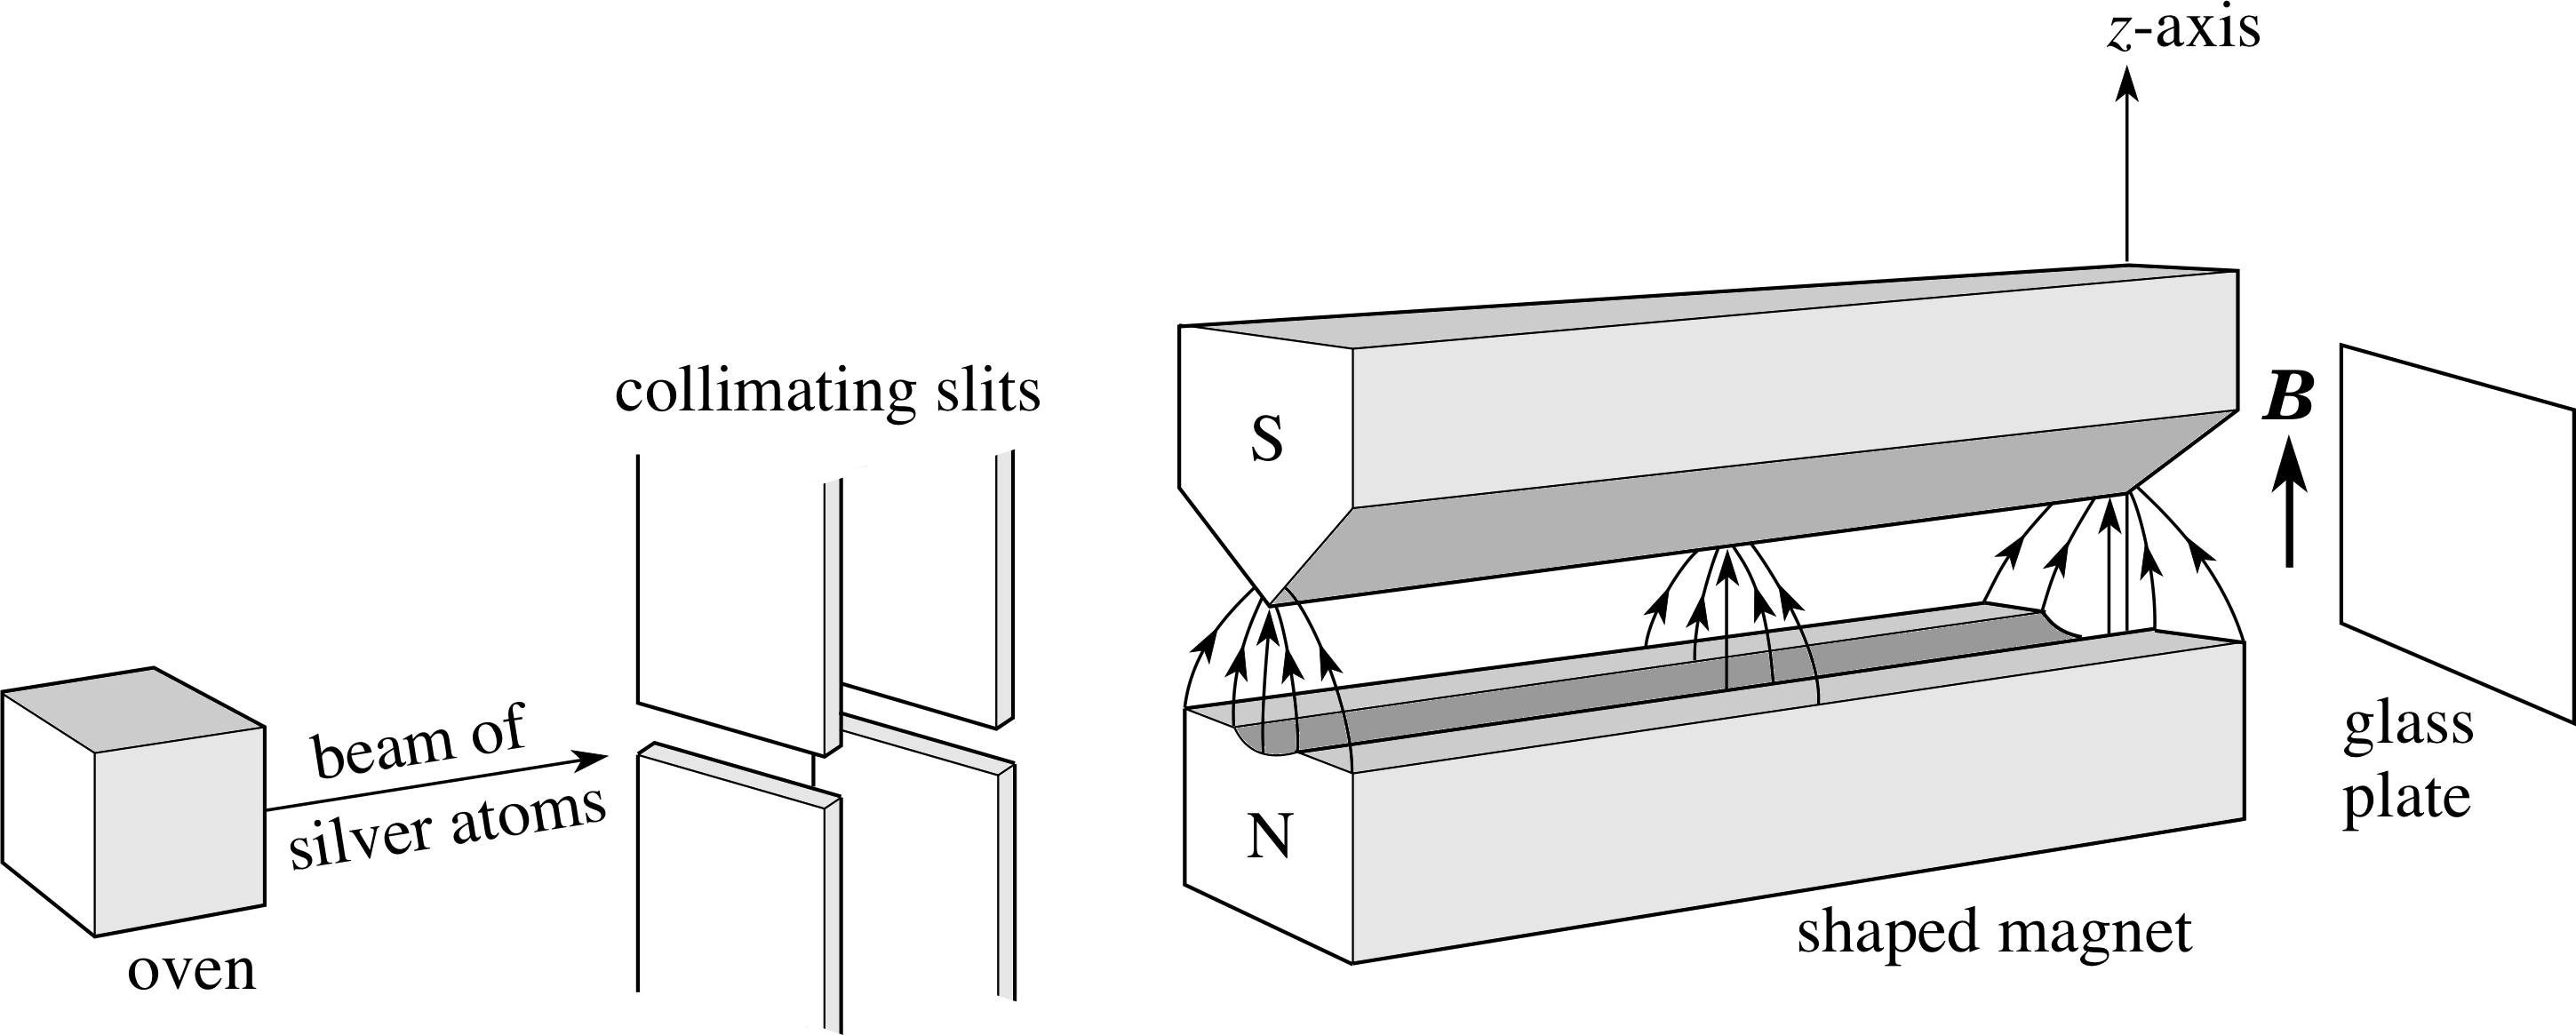
\includegraphics[width=0.7\linewidth]{files/S_G_experiment-437e0363a97a3f51196848de1f7c3d55.png}
\end{figure}

We want to know where would the silver atoms land on the glass plate. First we analyze through classical electromagnetics:

\begin{theorem}The potential energy of interaction between a \textbf{magnetic dipole}($\boldsymbol{\mu}$)and the \textbf{magnetic field}($\mathbf{B}$) is :
\begin{equation}
U = -\boldsymbol{\mu}\cdot \mathbf{B}
\end{equation}

\end{theorem}Since the energy is lowered if the dipole aligns with the magnetic field. As a result, the force experienced by the the dipole is simply:
\begin{equation}
\nabla U=-\nabla(\boldsymbol{\mu}\cdot \mathbf{B})
\end{equation}

In particular, we get that the $z$ component of the force is :

\begin{equation}
F^{(z)}&= -\partial_z (\mu^{(z)} B^{x}+ \mu^{(x)} B^{z} +\mu^{(y)} B^{y})
\end{equation}

In our case,




\end{document}
